% !TeX spellcheck = en_US
\chapter{Implementation and Validation}%

The first step of the validation involves constructing a basic model that captures the kinematics and dynamics of an industrial robot. To test the method in a simple case, the first tests are performed on a 6-DoF model and a 5-DoF toolpath. The sixth DoF (rotation around Z) is freely defined and is used for the optimzation. After the validation on this simple model, an additional redundant DoF is introduced in form of a rotary-tilt table. 

Once the basic mathematical model is established, a optimization algorithm is implemented to determine the optimal values for each parameter associated with the redundant DoF. These methods and optimization algorithms can consider the industrial robot's specific objectives and constraints, like for example, minimizing direction changes or joint accelerations. 

%After that, the goal is to incorporate this method with a selected CAM software to be tested in more complex scenarios.


\section{Simple Implementation}%
\subsection{Modeling a 6-DoF robot}
In order to test the proposed method, a simple articulated 6-DoF industrial robot is used as a model. A visualization of that robot is given in figure \ref{robotprog}. The Denavit-Hartenberg (DH) parameters for this robot can be found in Table \ref{DH}.

\begin{table}[H]
	\centering
	\begin{tabular}{||l|l||}
		  & Values \\
		\hline
		\hline
		\hline
		a	&		[200, 900, 150, 0,   150, 0] \\
		alpha	&  	[90,  0,   90,  -90, 90,  -90] \\
		d	& 		[600  0,   0,   800, 0,   200]\\
		
		\hline
		\hline
	\end{tabular}
	
	\caption{DH-parameters for the modeled robot}
	\label{DH}
\end{table}

These parameters describe the geometry and kinematics of a robotic arm. They are used to define the relationship between adjacent links in a robot's kinematic chain. The DH parameters include values such as link lengths, link twists and link offsets. In this model, "a" represents the link lengths between adjacent joints, "alpha" represents the link twists or rotations around the Z-axis between adjacent joints and "d" represents the link offsets or distances along the Z-axis between adjacent joints. 
It is important to note that the last rotation is defined in the negative direction. This is done to ensure that the end of the last joint can be perceived as the tip of a tool without the need for any extra transformations.
Figure \ref{robotprog} shows the robot modeled in Python. The joint positions are [  2,  75, -45,  -88, -91,  61] in degrees, for joint 1 to 6 respectively.

 \begin{figure}[H]
	\centerline{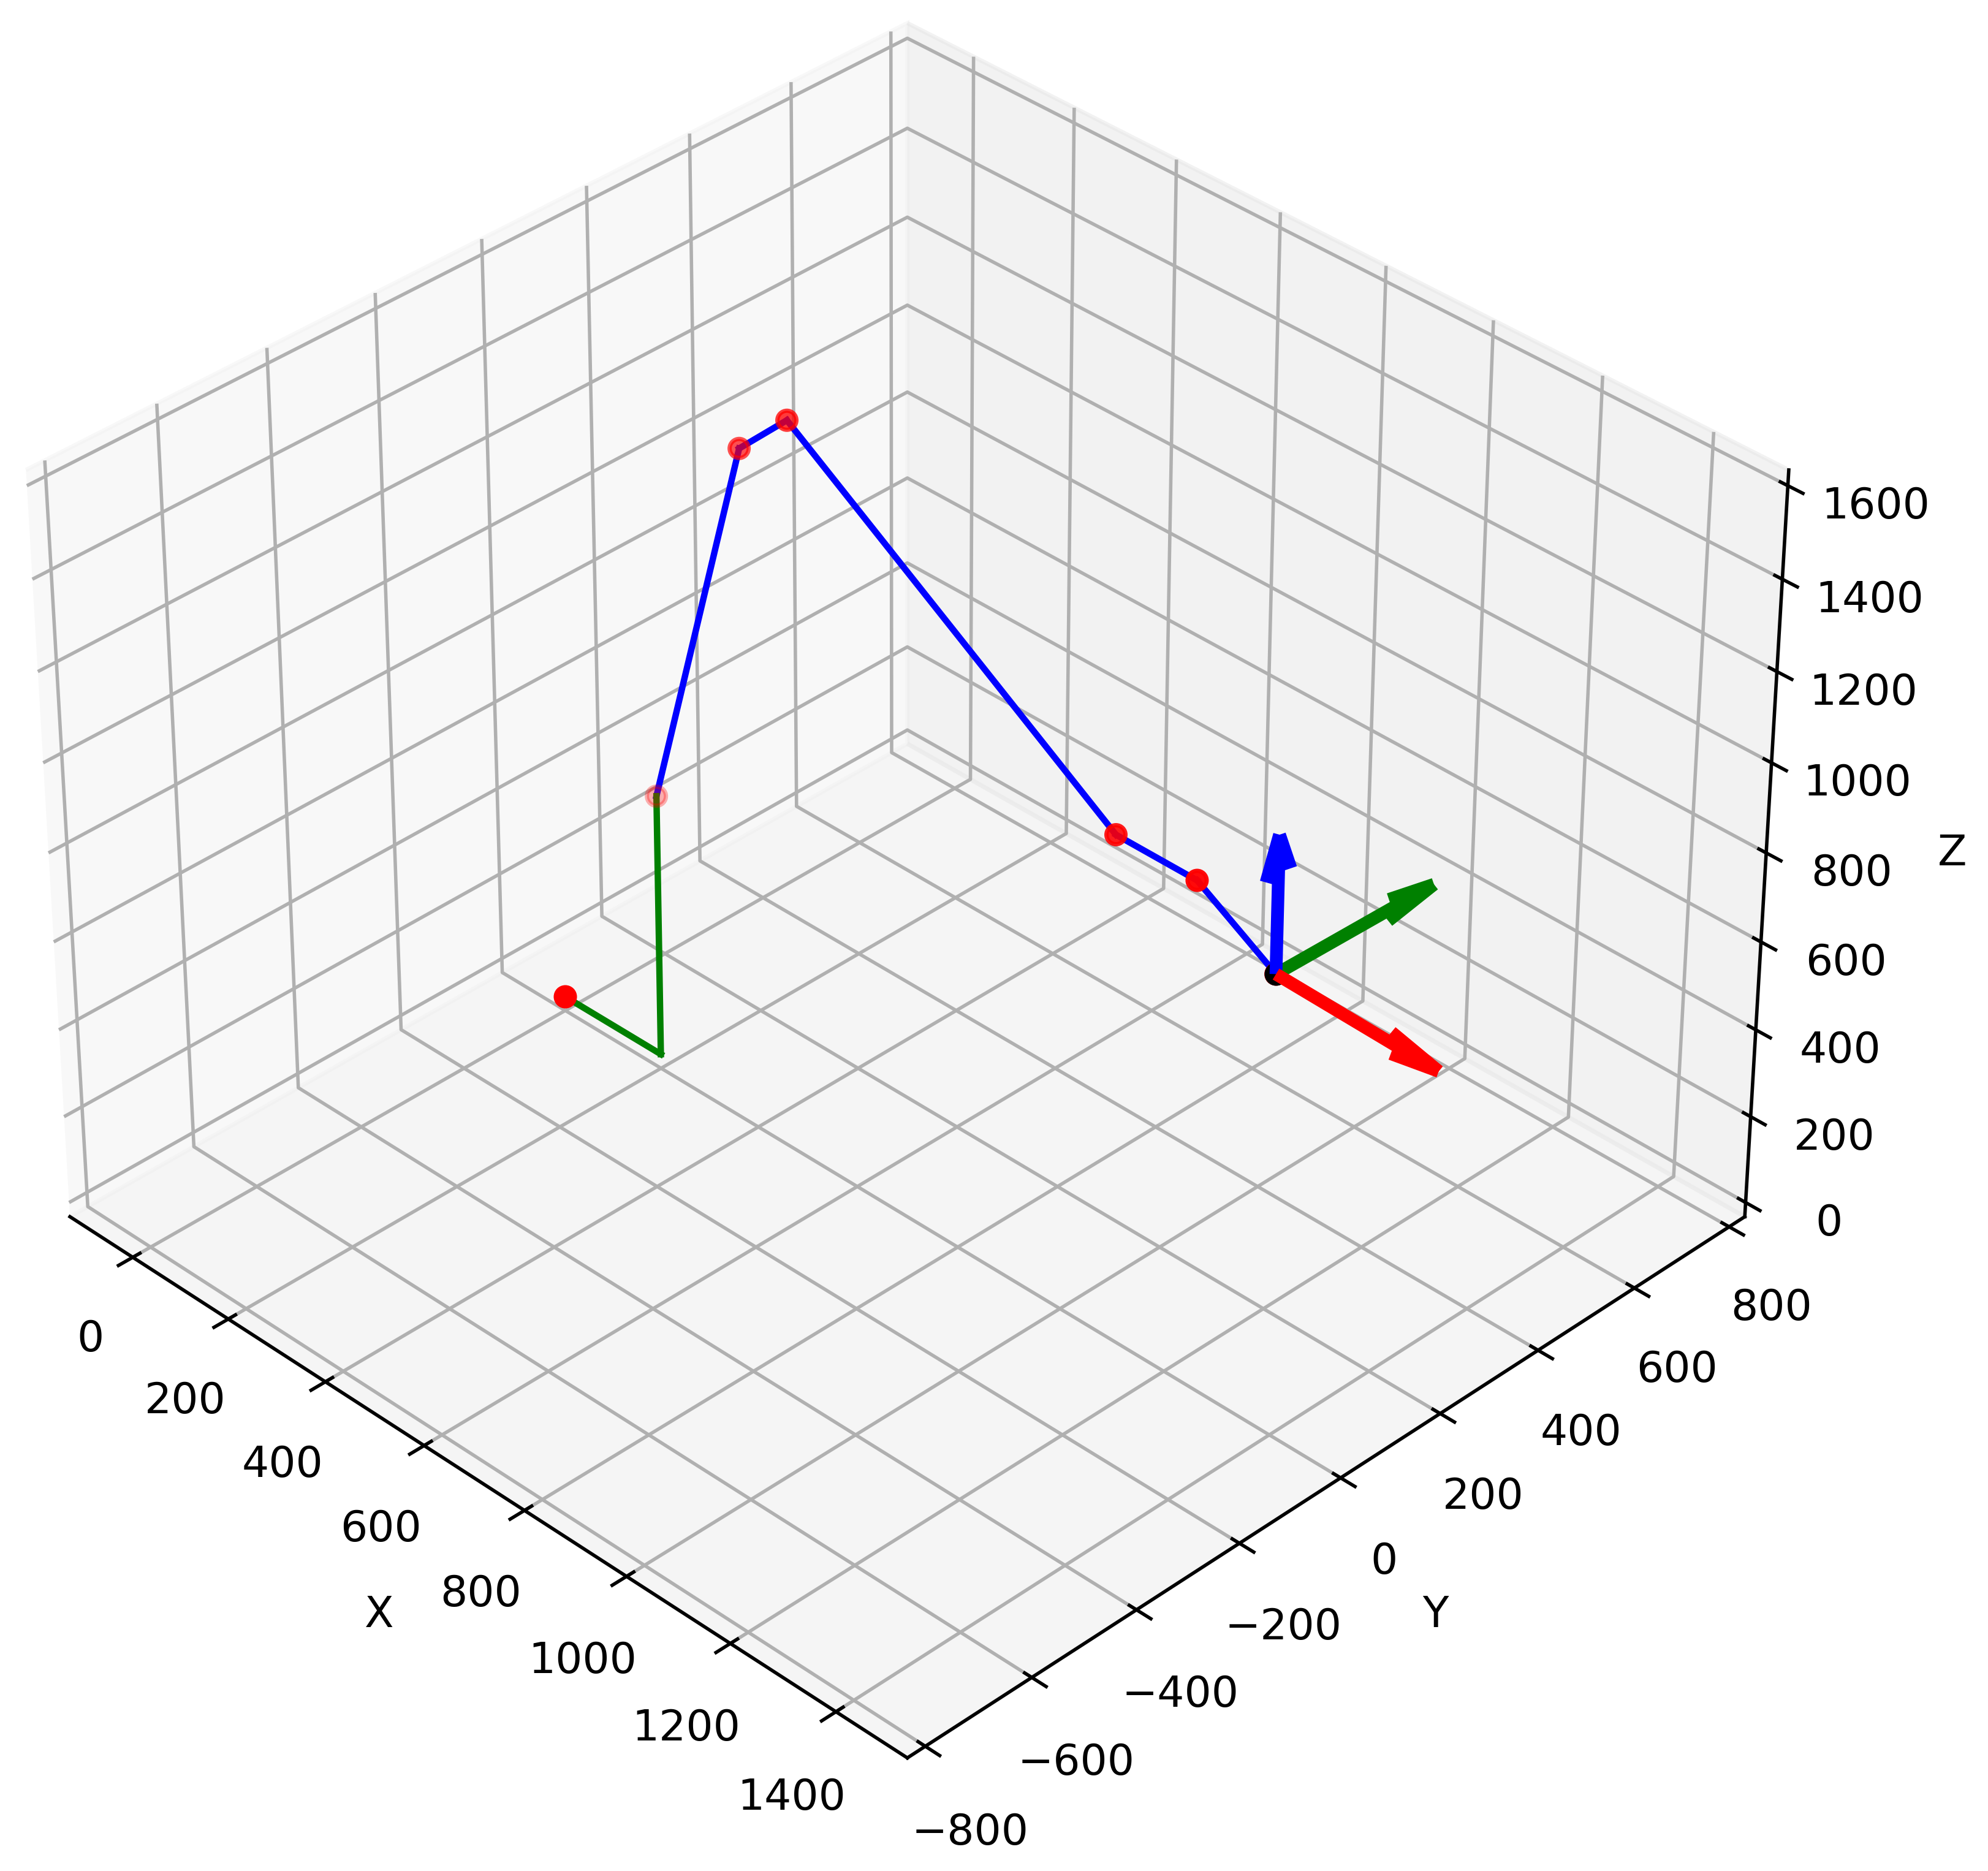
\includegraphics[width=0.9\textwidth]{figures/robotprog.png}}
	\caption{Visualization of the modeled robot}
	\label{robotprog}
\end{figure}


The arrows represent the coordinate axis of the TCP. For simplicity, the TCP is equal to the end point of the last joint. The X-axis is shown in red while the green and blue are the Y-axis and Z-axis respectively. The first link is shown in green and originates at the point~X=0~Y=0~Z=0.


The schematic of the modeled robot is shown in Figure \ref{schema}. In this configuration, all joints are in their initial position without any rotation.
\begin{figure}[H]
	\centerline{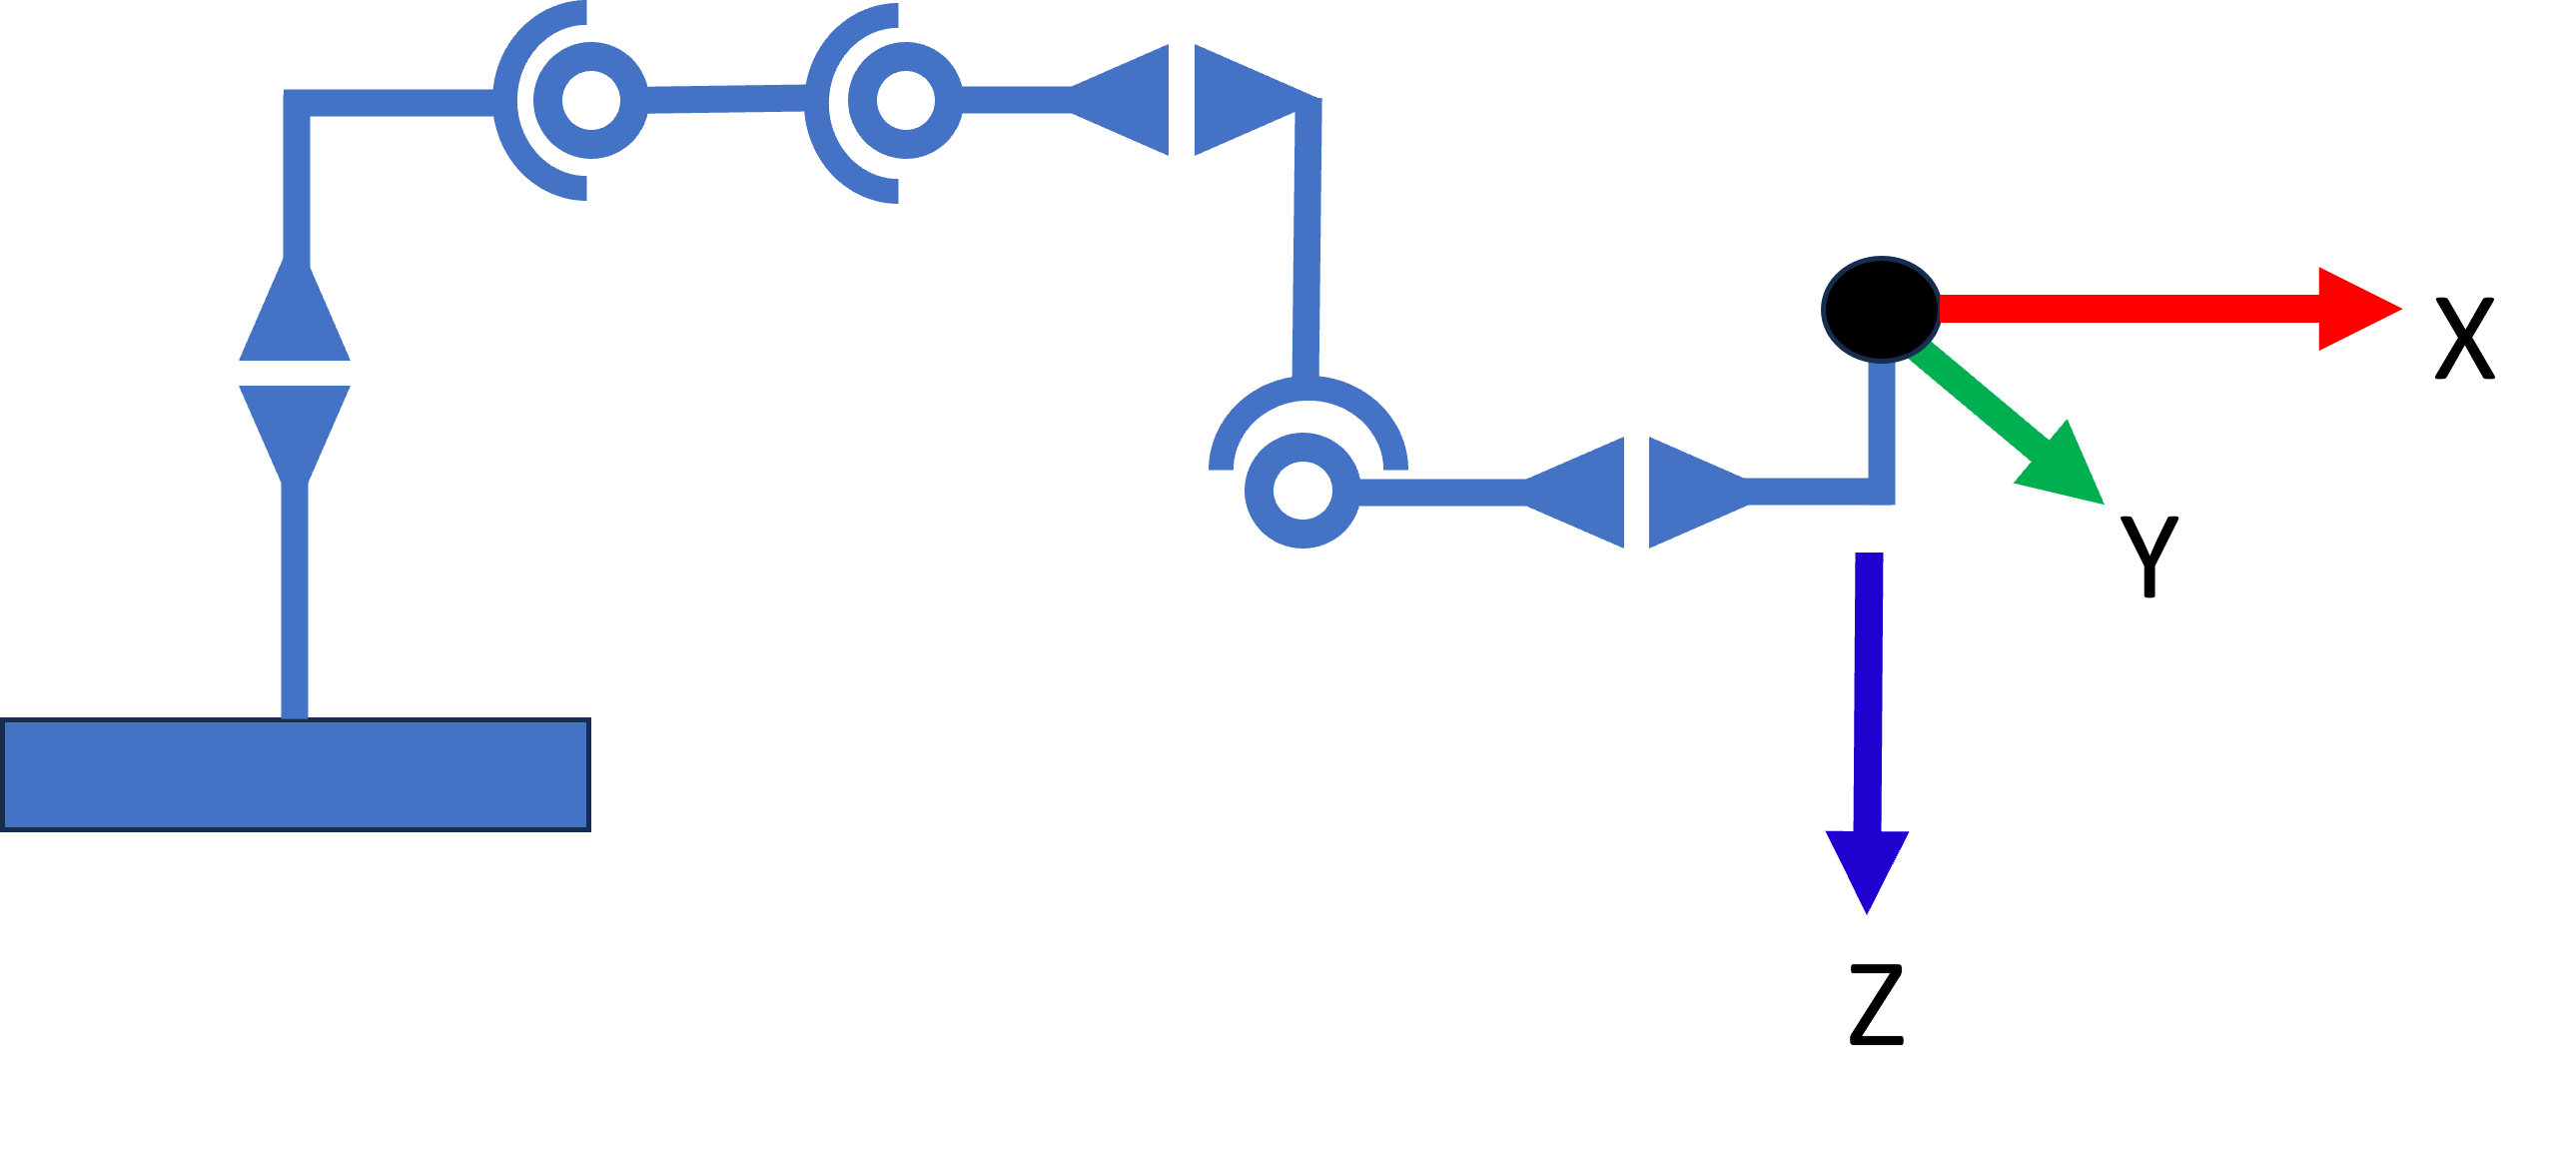
\includegraphics[width=0.7\textwidth]{figures/schema.png}}
	\caption{Schematics of the modeled robot}
	\label{schema}
\end{figure}

\subsection{Modeling a basic Toolpath}\label{MBT}
Before the process parameters can be analyzed, a toolpath needs to be defined for the TCP to follow. In this particular case, three possible options are presented. Each toolpath consists of 3000 coordinates. It is important to note that in these cases, the redundant DoF is the rotation around the Z-Axis. This means that  this rotation will be adjusted to identify the most optimal value for the desired outcome.


The first toolpath, shown in Figure \ref{path1}, depicts a converging-diverging spiral. Figure \ref{path2} illustrates a converging infinity-loop, and Figure \ref{path3} displays a forward-moving sinusoidal curve. 

The corresponding equations are represented by Equation~\ref{eq1}, Equation~\ref{eq2}, and Equation~\ref{eq3}. The variable \textit{iter} increments from 0 to 3000 and is used to calculate the X-Y-Z coordinates. The trigonometric functions are implemented using the \textit{Numpy} library. No rotation (A,B~or~C) is defined so far. Only the coordinates are specified. All toolpaths have specifically selected dimensions and characteristics. Toolpath 1 and 2 are continuous while toolpath 3 has abrupt direction changes. Only toolpath 1 has rotational symmetry. 


\begin{equation}\label{eq1}
\begin{split}
x &= np.cos(np.deg2rad(iter)) * (500 - iter / 3)\\
y &= np.sin(np.deg2rad(iter)) * (500 - iter / 3)\\
z &= iter / 10
\end{split}
\end{equation}


\begin{equation}\label{eq2}
\begin{split}
x &= np.sin(np.deg2rad(iter)) * (400-iter / 5)\\
y &= np.sin(np.deg2rad(iter)) * np.cos(np.deg2rad(iter)) * (500-iter / 6)\\
z &= iter / 10
\end{split}
\end{equation}

\begin{equation}\label{eq3}
\begin{split}
x &= np.sin(np.deg2rad(iter)) * 200\\
y &= iter / 3 - (2500/6)\\
z &= np.sin(np.deg2rad(x))*100
\end{split}
\end{equation}


\begin{figure}[H]% [H] is so declass\'e!
	\centering
	\begin{minipage}{0.5\textwidth}
		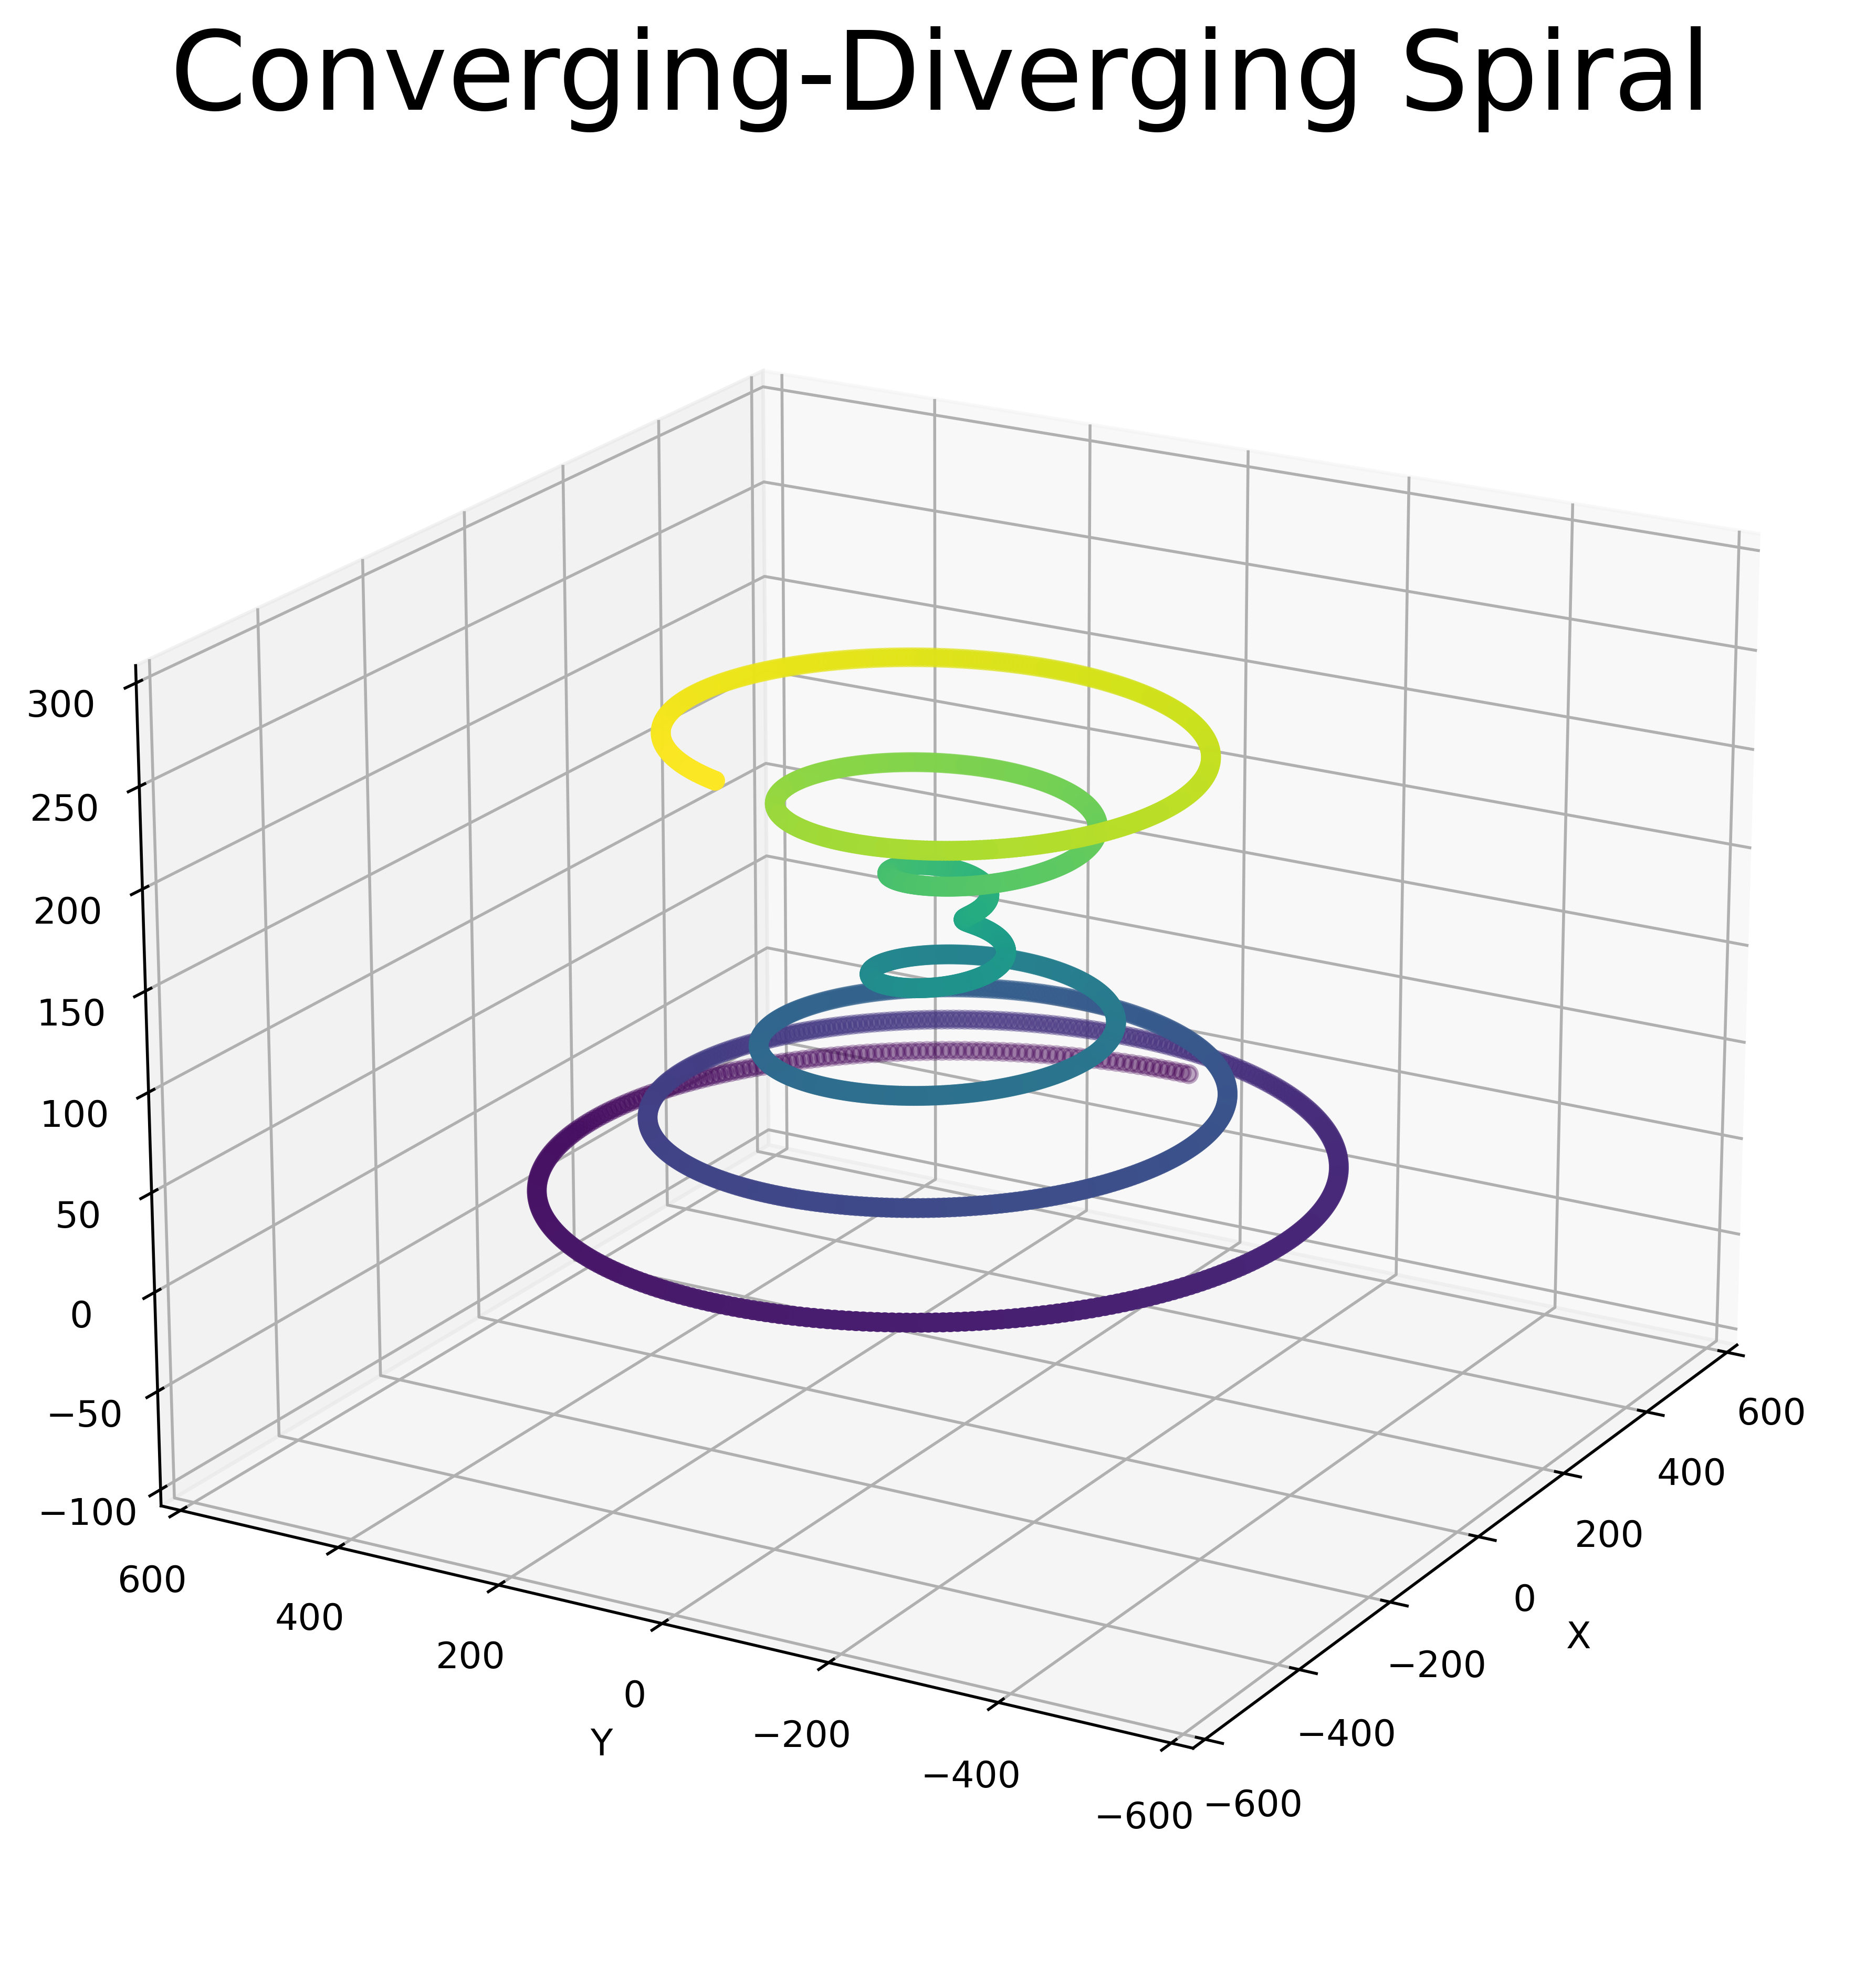
\includegraphics[width=\textwidth]{figures/path1.png}
		\caption{Toolpath 1: Converging-Diverging Spiral}
		\label{path1}
	\end{minipage}\hfill
	\begin{minipage}{0.5\textwidth}
		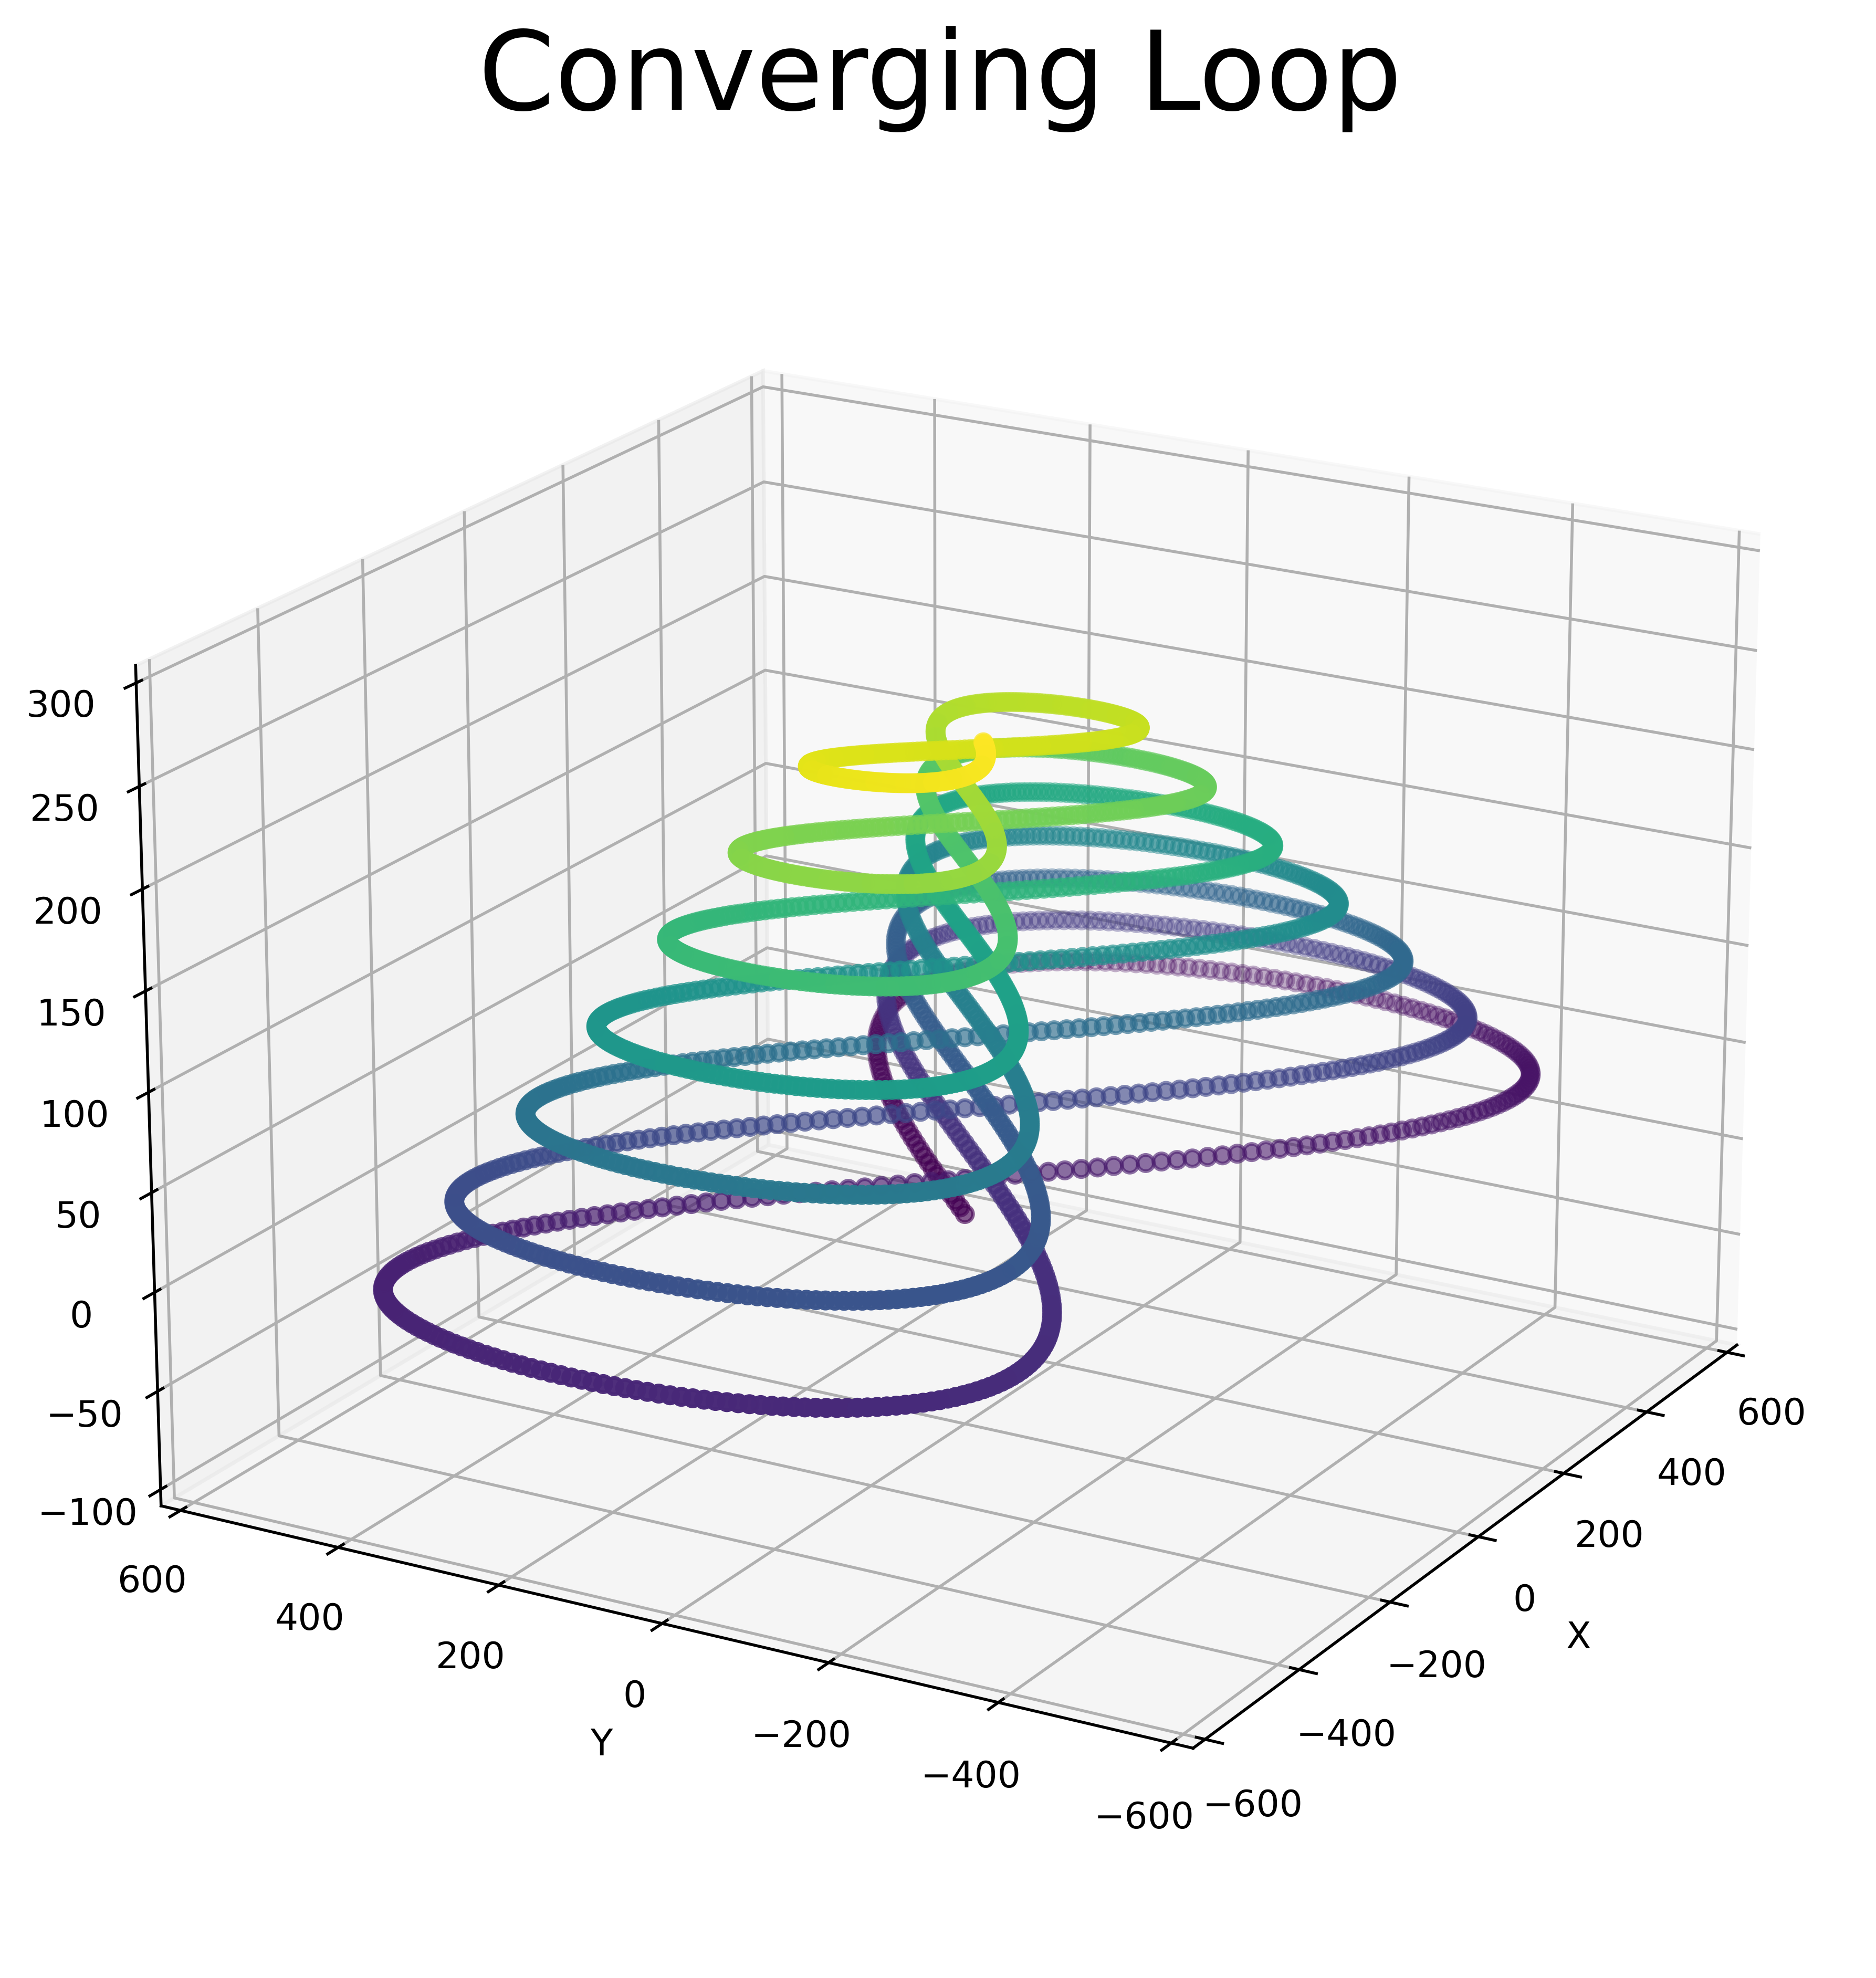
\includegraphics[width=\textwidth]{figures/path2.png}
		\caption{Toolpath 2: Converging Loop}
		\label{path2}
	\end{minipage}\par
	\vskip\floatsep% normal separation between figures
	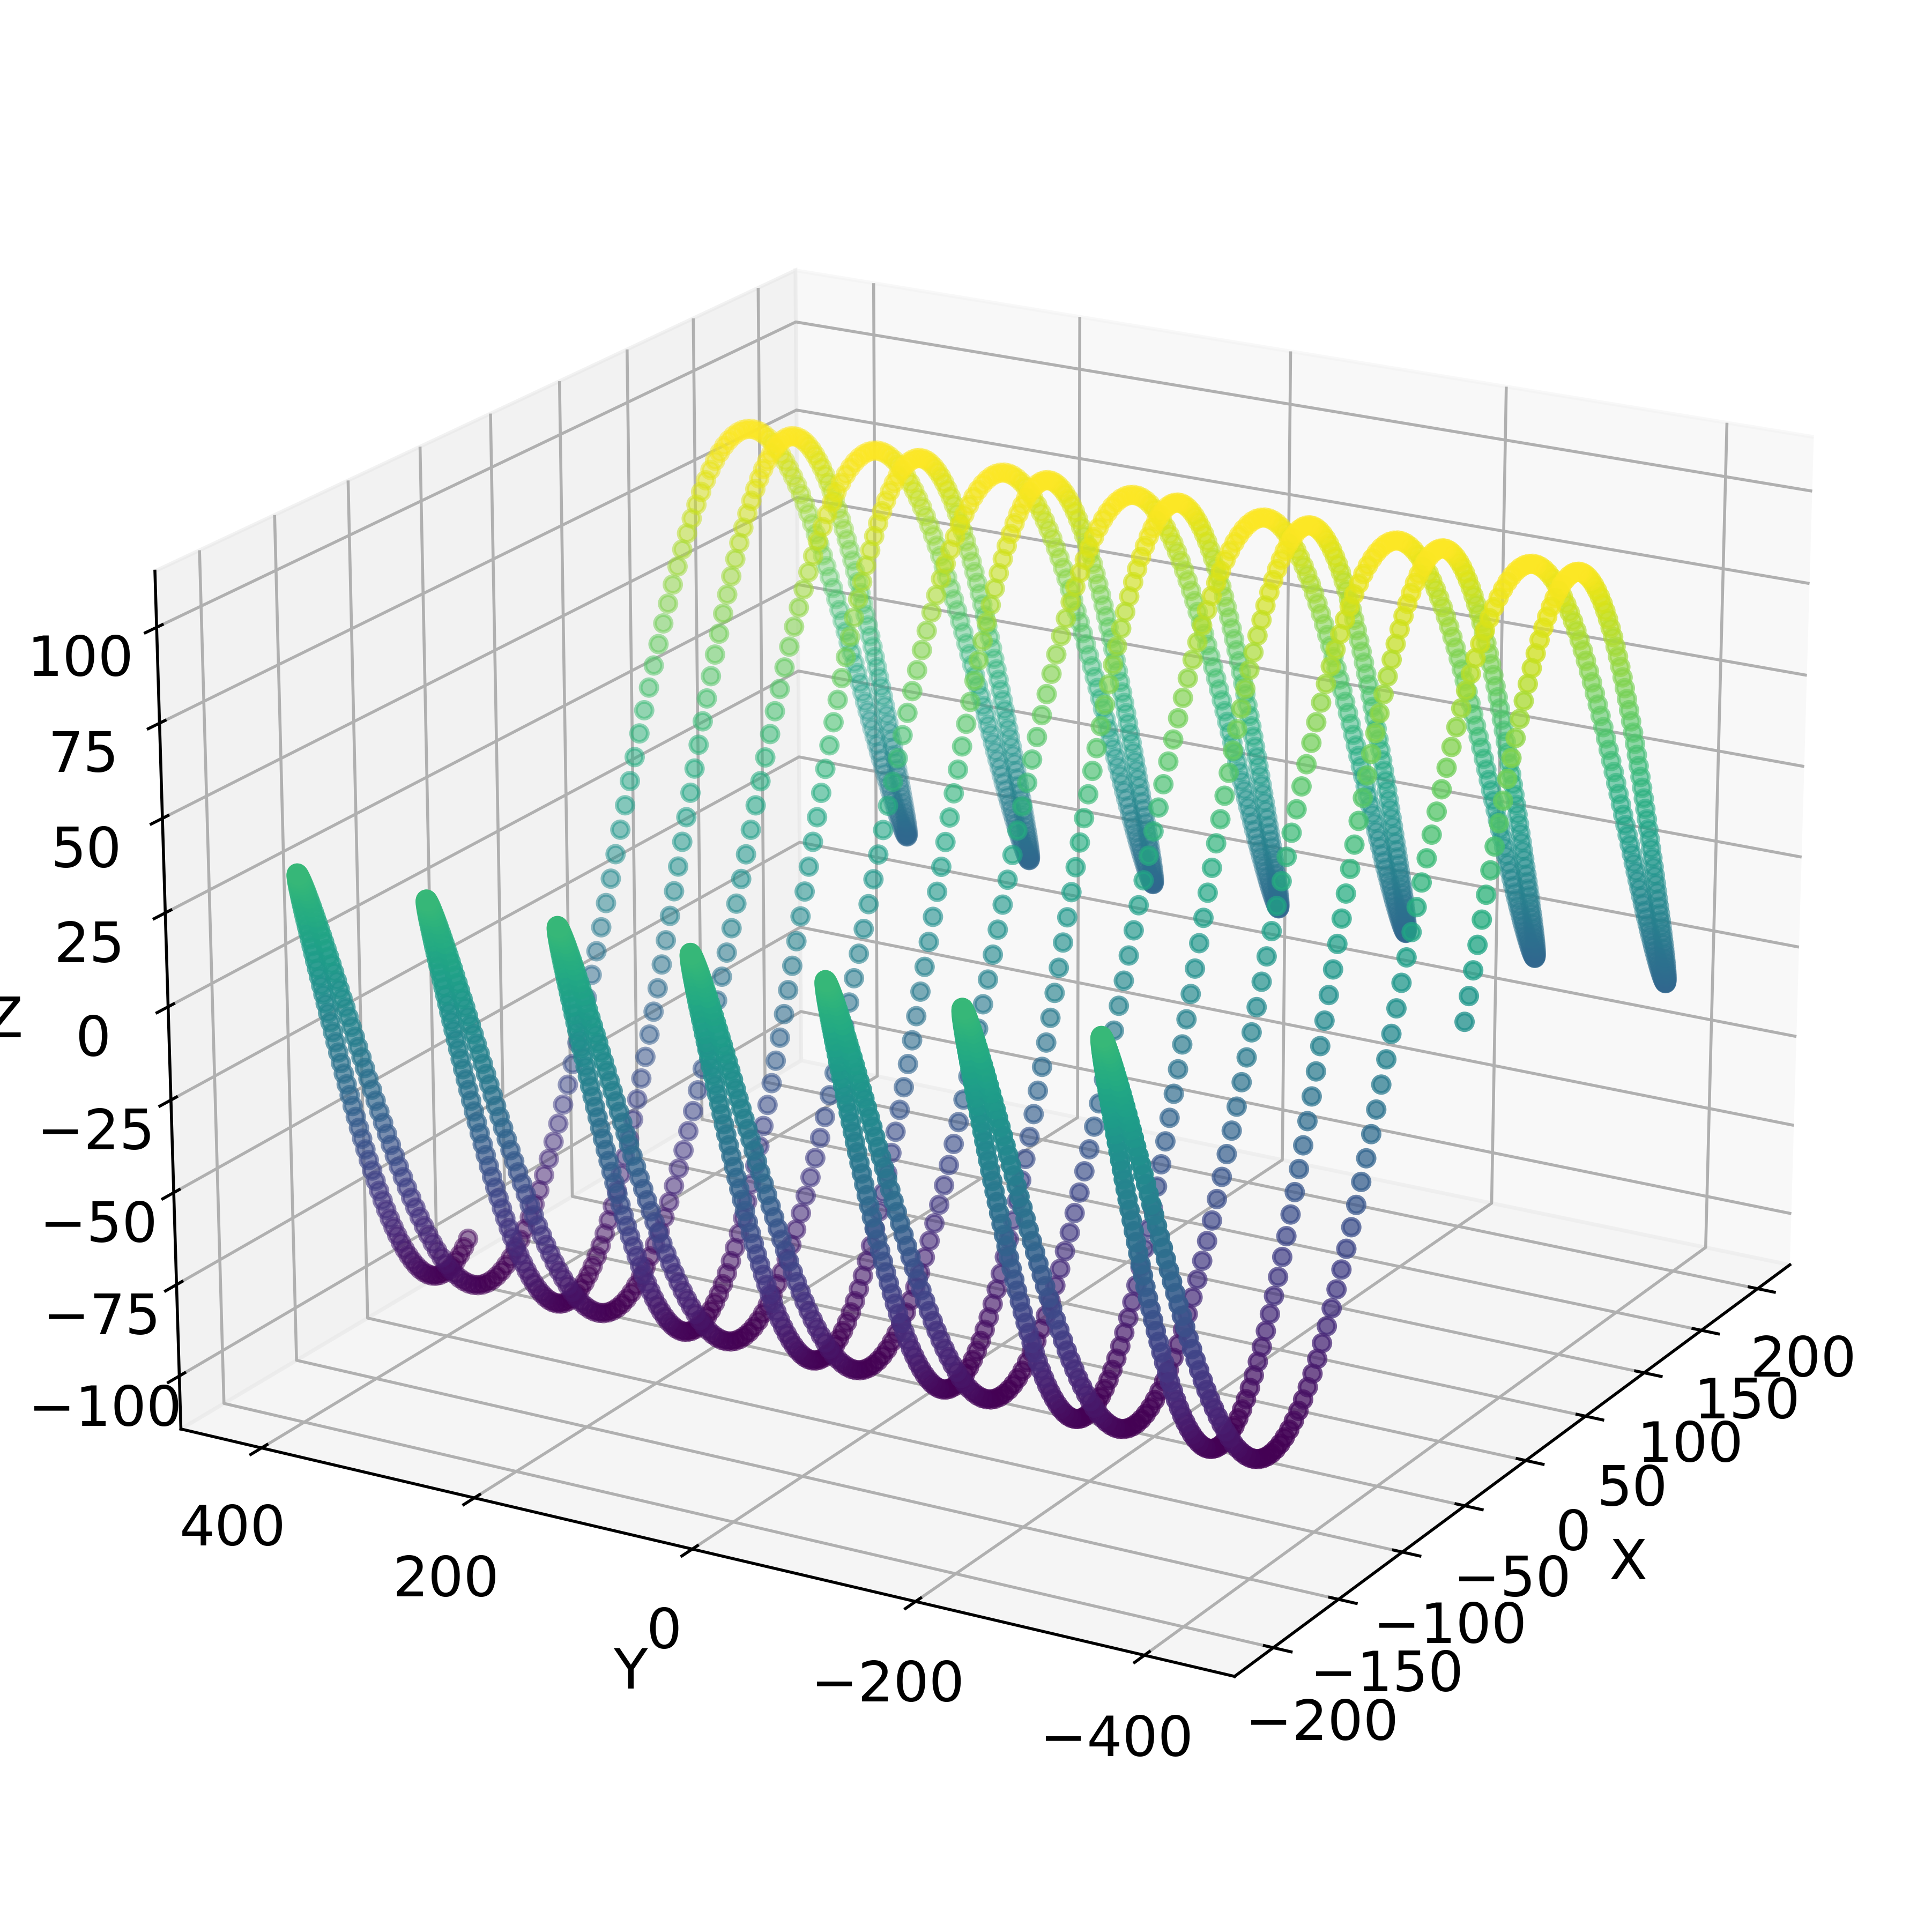
\includegraphics[width=0.5\textwidth]{figures/path3.png}

	\caption{Toolpath 3: Pendulum Oscillation}
	\label{path3}
\end{figure}

\newpage
Figure \ref{TP1robot} depicts the robot and Toolpath 1 (described by Equation \ref{eq1}) at the final position of the toolpath. The toolpath's origin is shifted by X=1000 and Z=600 relative to the robot's coordinate system. There is no rotation around axes X, Y, and Z. Thus A B and C is zero.
The coordinate axis of the toolpath are parallel to the axis of the robots coordinate system.



\begin{figure}[H]
	\centerline{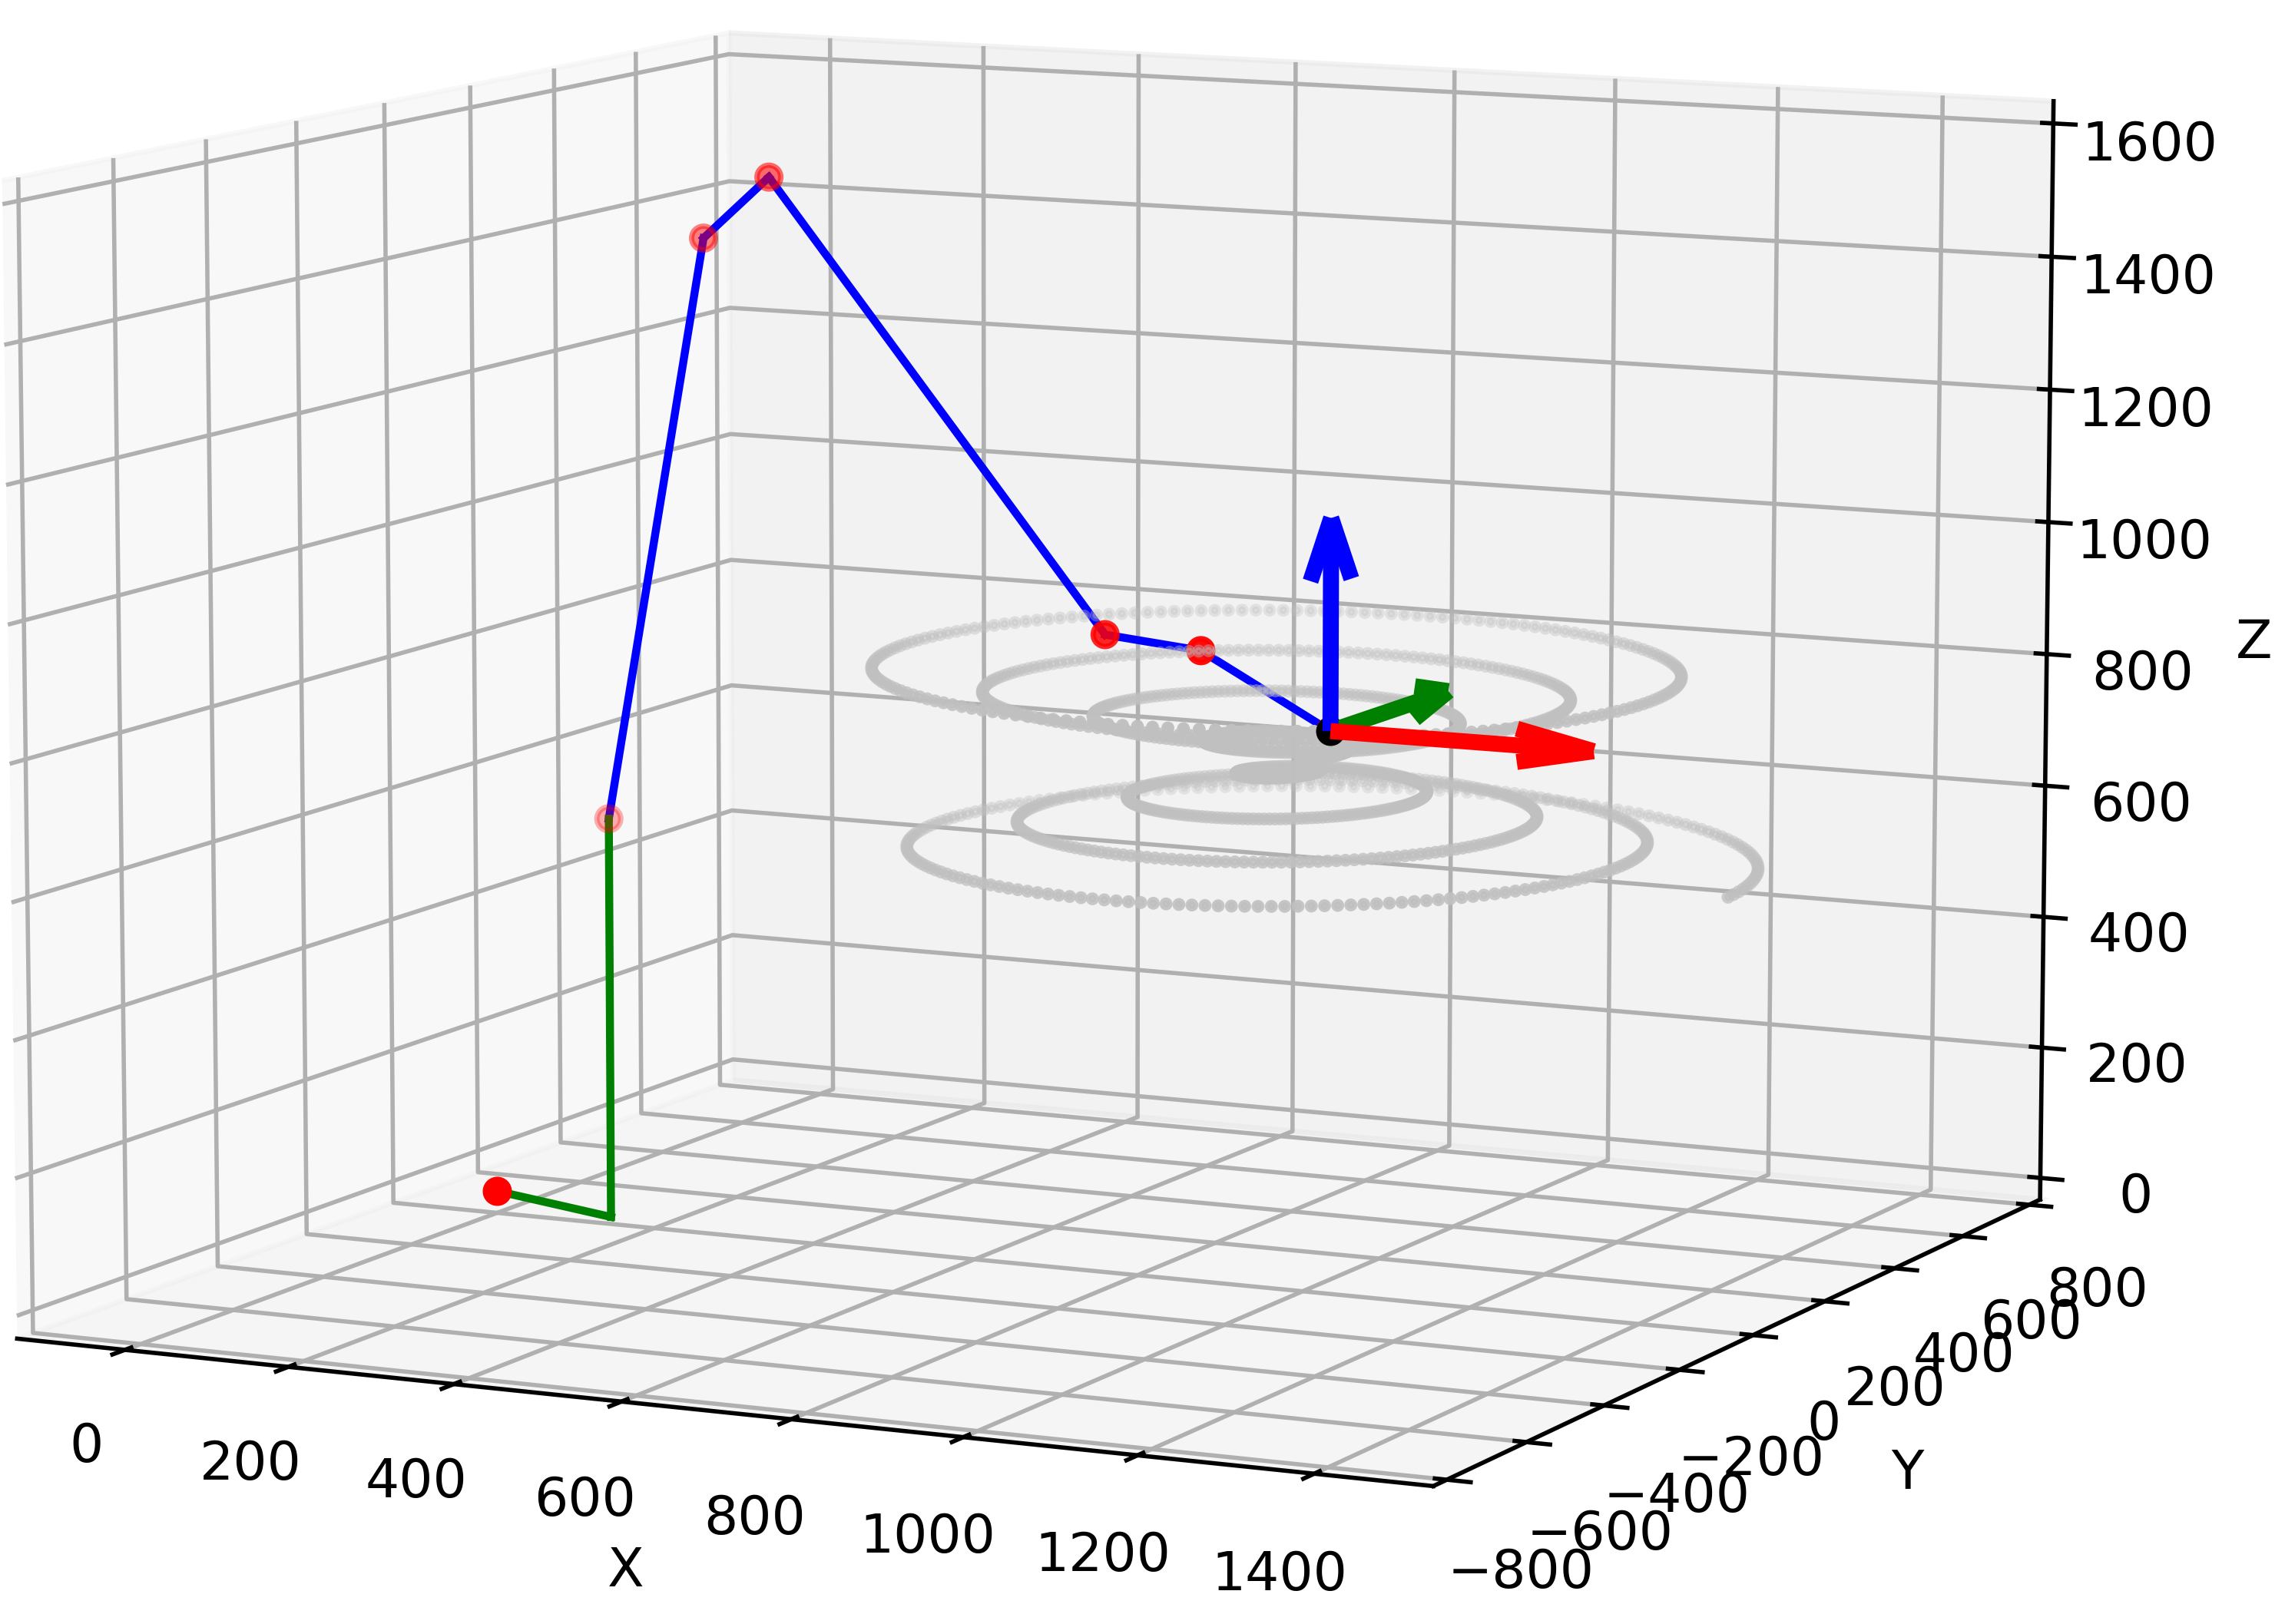
\includegraphics[width=0.9\textwidth]{figures/robotANDpath1.png}}
	\caption{Toolpath 1 with robot model}
	\label{TP1robot}
\end{figure}




\subsection{Extracting process parameters}
With the assistance of an inverse kinematics algorithm from the Python library \textit{visual\_kinematics}, the joint angles for each coordinate can be computed. For that the rotation A, B and C need to be defined. The outcome is a time series containing the corresponding joint positions. Currently, all coordinates must be traversed in equidistant timesteps. With this information, it becomes feasible to calculate the velocity and other related parameters. After transforming all the data from the time series into scalar values and calculating the local score, the global score can be determined.
\newpage
\section{Testing and Validation}%

\subsection{Toolpath Evaluation with one Redundant DoF}
%\subsubsection{Obtaining Joint Positions}
As mentioned in Chapter \ref{MBT}, the toolpath is considered constant in regards to the coordinates X-Y-Z. The fixed boundary conditions for the robot are that the rotations around the X and Y axes are 0. Thus A and B are both equal to zero. The user needs to set the DoF for the rotation around the Z axis, which is the redundant DoF. Figure \ref{TP1ABC0} illustrates the variation of each joint over time for toolpath 1. In this specific case, the rotations A, B, and C are set to~0. The whole toolpath is traversed in 300 seconds. 

\begin{figure}[H]
	\centerline{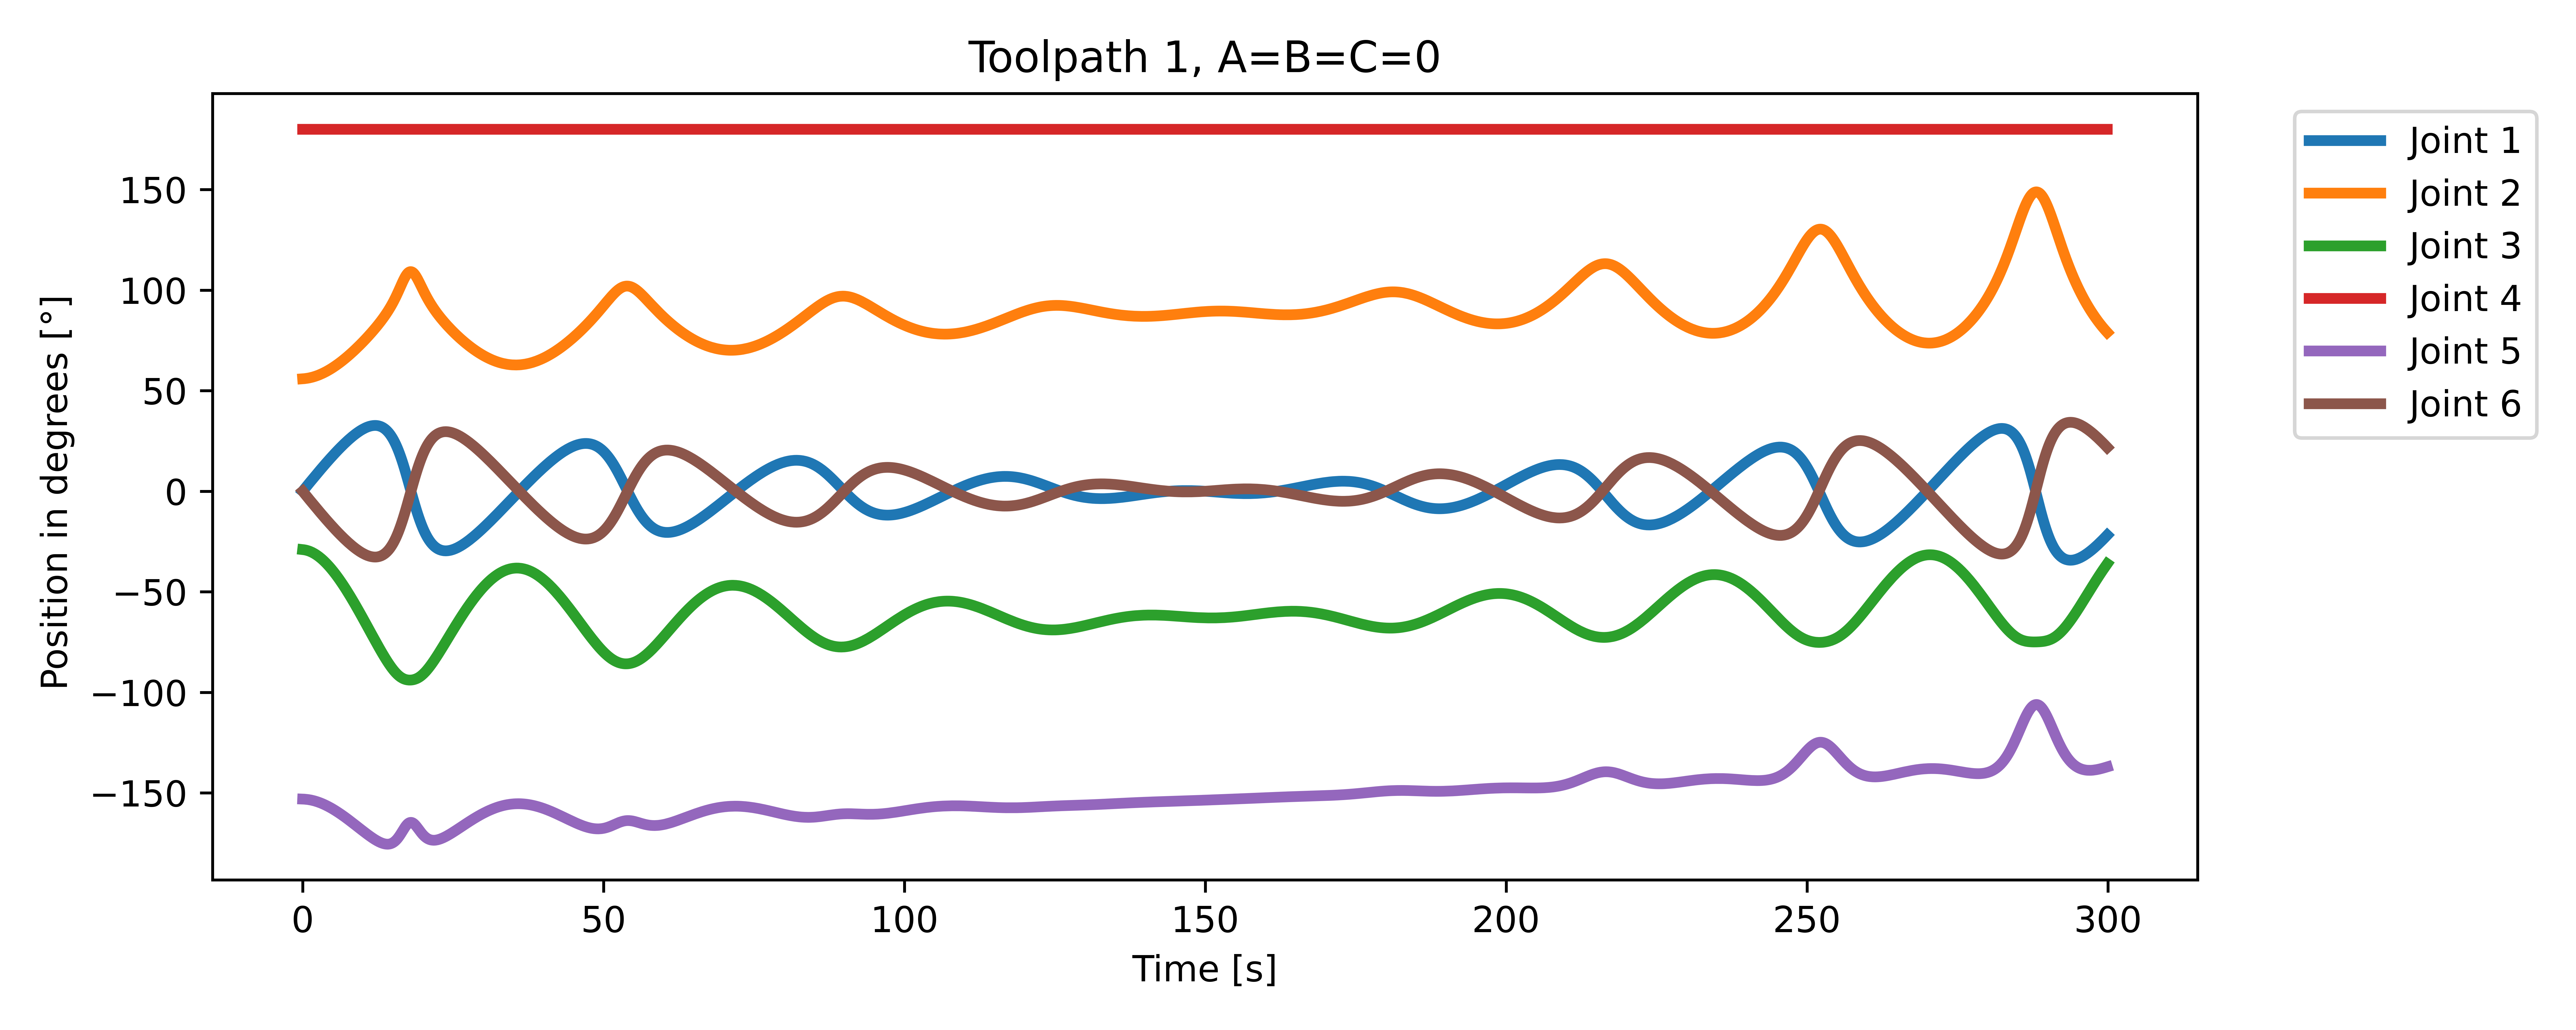
\includegraphics[width=1\textwidth]{figures/TP1ABC0.png}}
	\caption{Visualization of the joint positions over time for toolpath 1 with C=0}
	\label{TP1ABC0}
\end{figure}

Figure \ref{TP1ABC45} illustrates the positions of the joints over time for the toolpath, with a 45° rotation around the Z-axis (C = 45°). It is evident that joint 4 and 5 have experienced a change in their respective ranges. Additionally, joint 6 displays a considerably larger amplitude towards the end of the toolpath, compared to no rotation (C=0).

\begin{figure}[H]
	\centerline{\includegraphics[width=1\textwidth]{figures/TP1ABC45.png}}
	\caption{Visualization of the joint positions over time for toolpath 1 with C=45°}
	\label{TP1ABC45}
\end{figure}


%Joints 1 and 6 oscillate out of phase relative to each other around a zero degrees. Joint 3 remains constantly at 180 degrees. Joint 2 and 5 also oscillate and slightly increase.

Figure \ref{TP1ABC0} depicts the changes in each joint over time for toolpath 2 (Eq. \ref{eq2}) with no rotation. In contrast to toolpath 1, the amplitudes decrease notably towards the end of the toolpath. This observation aligns with the distinct characteristics of different toolpaths.
 
 %In this case all joints show a oscillation except joint 4.
\begin{figure}[H]
	\centerline{\includegraphics[width=1\textwidth]{figures/TP2ABC0.png}}
	\caption{Visualization of the joint positions over time for toolpath 2}
	\label{TP2ABC0}
\end{figure}

%ToDo: EXPLAIN WHY JOINT 4 IS AT 180 all the time!!!!!!!!\newline
%\subsubsection{Selecting Process Parameters}
The next step is to select the process parameter of interest and establish their respective weights. For that, a basic case is discussed. The selected process parameters can be found in table \ref{PPbasic}. The total number of direction changes in all joints and the total distance traveled are selected due to the simplicity in their implementation.

The number of direction changes is given an importance rating of 0.2.
The total travel has a importance factor of 0.4. Additionally, the acceleration of joint 1 is analyzed. To obtain a scalar value for the acceleration, the individual values are squared and then summed up. The importance factor of the acceleration is 0.4.
Velocity, acceleration, and jerk are disregarded for all other joints.

\begin{table}[H]
	\centering
	\begin{tabular}{||l|l||}
		Process parameters& Importance Factor \\
		\hline
		\hline
		\hline
		Direction changes in joints 1-6	&		0.2 \\
		Total travel in joints 1-6	&  	0.4 \\
		Acceleration in joint 1	& 		0.4\\
		
		\hline
		\hline
	\end{tabular}
	
	\caption{Selected process parameters and their importance factors}
	\label{PPbasic}
\end{table}


As only a single DoF is being analyzed, it is possible to display the individual local scores and global score as a one-dimensional graph. Initially, toolpath 1 is analyzed, with the redundant DoF incremented by 5 degree staring at -135 and ending at 135 degrees. 
Figure \ref{TP1-25} and figure \ref{TP1+25} show two cases at -45 and +45 degrees of rotation around the Z-axis for toolpath 1.

\begin{figure}[H]
	\centering
	\begin{minipage}{0.5\textwidth}
		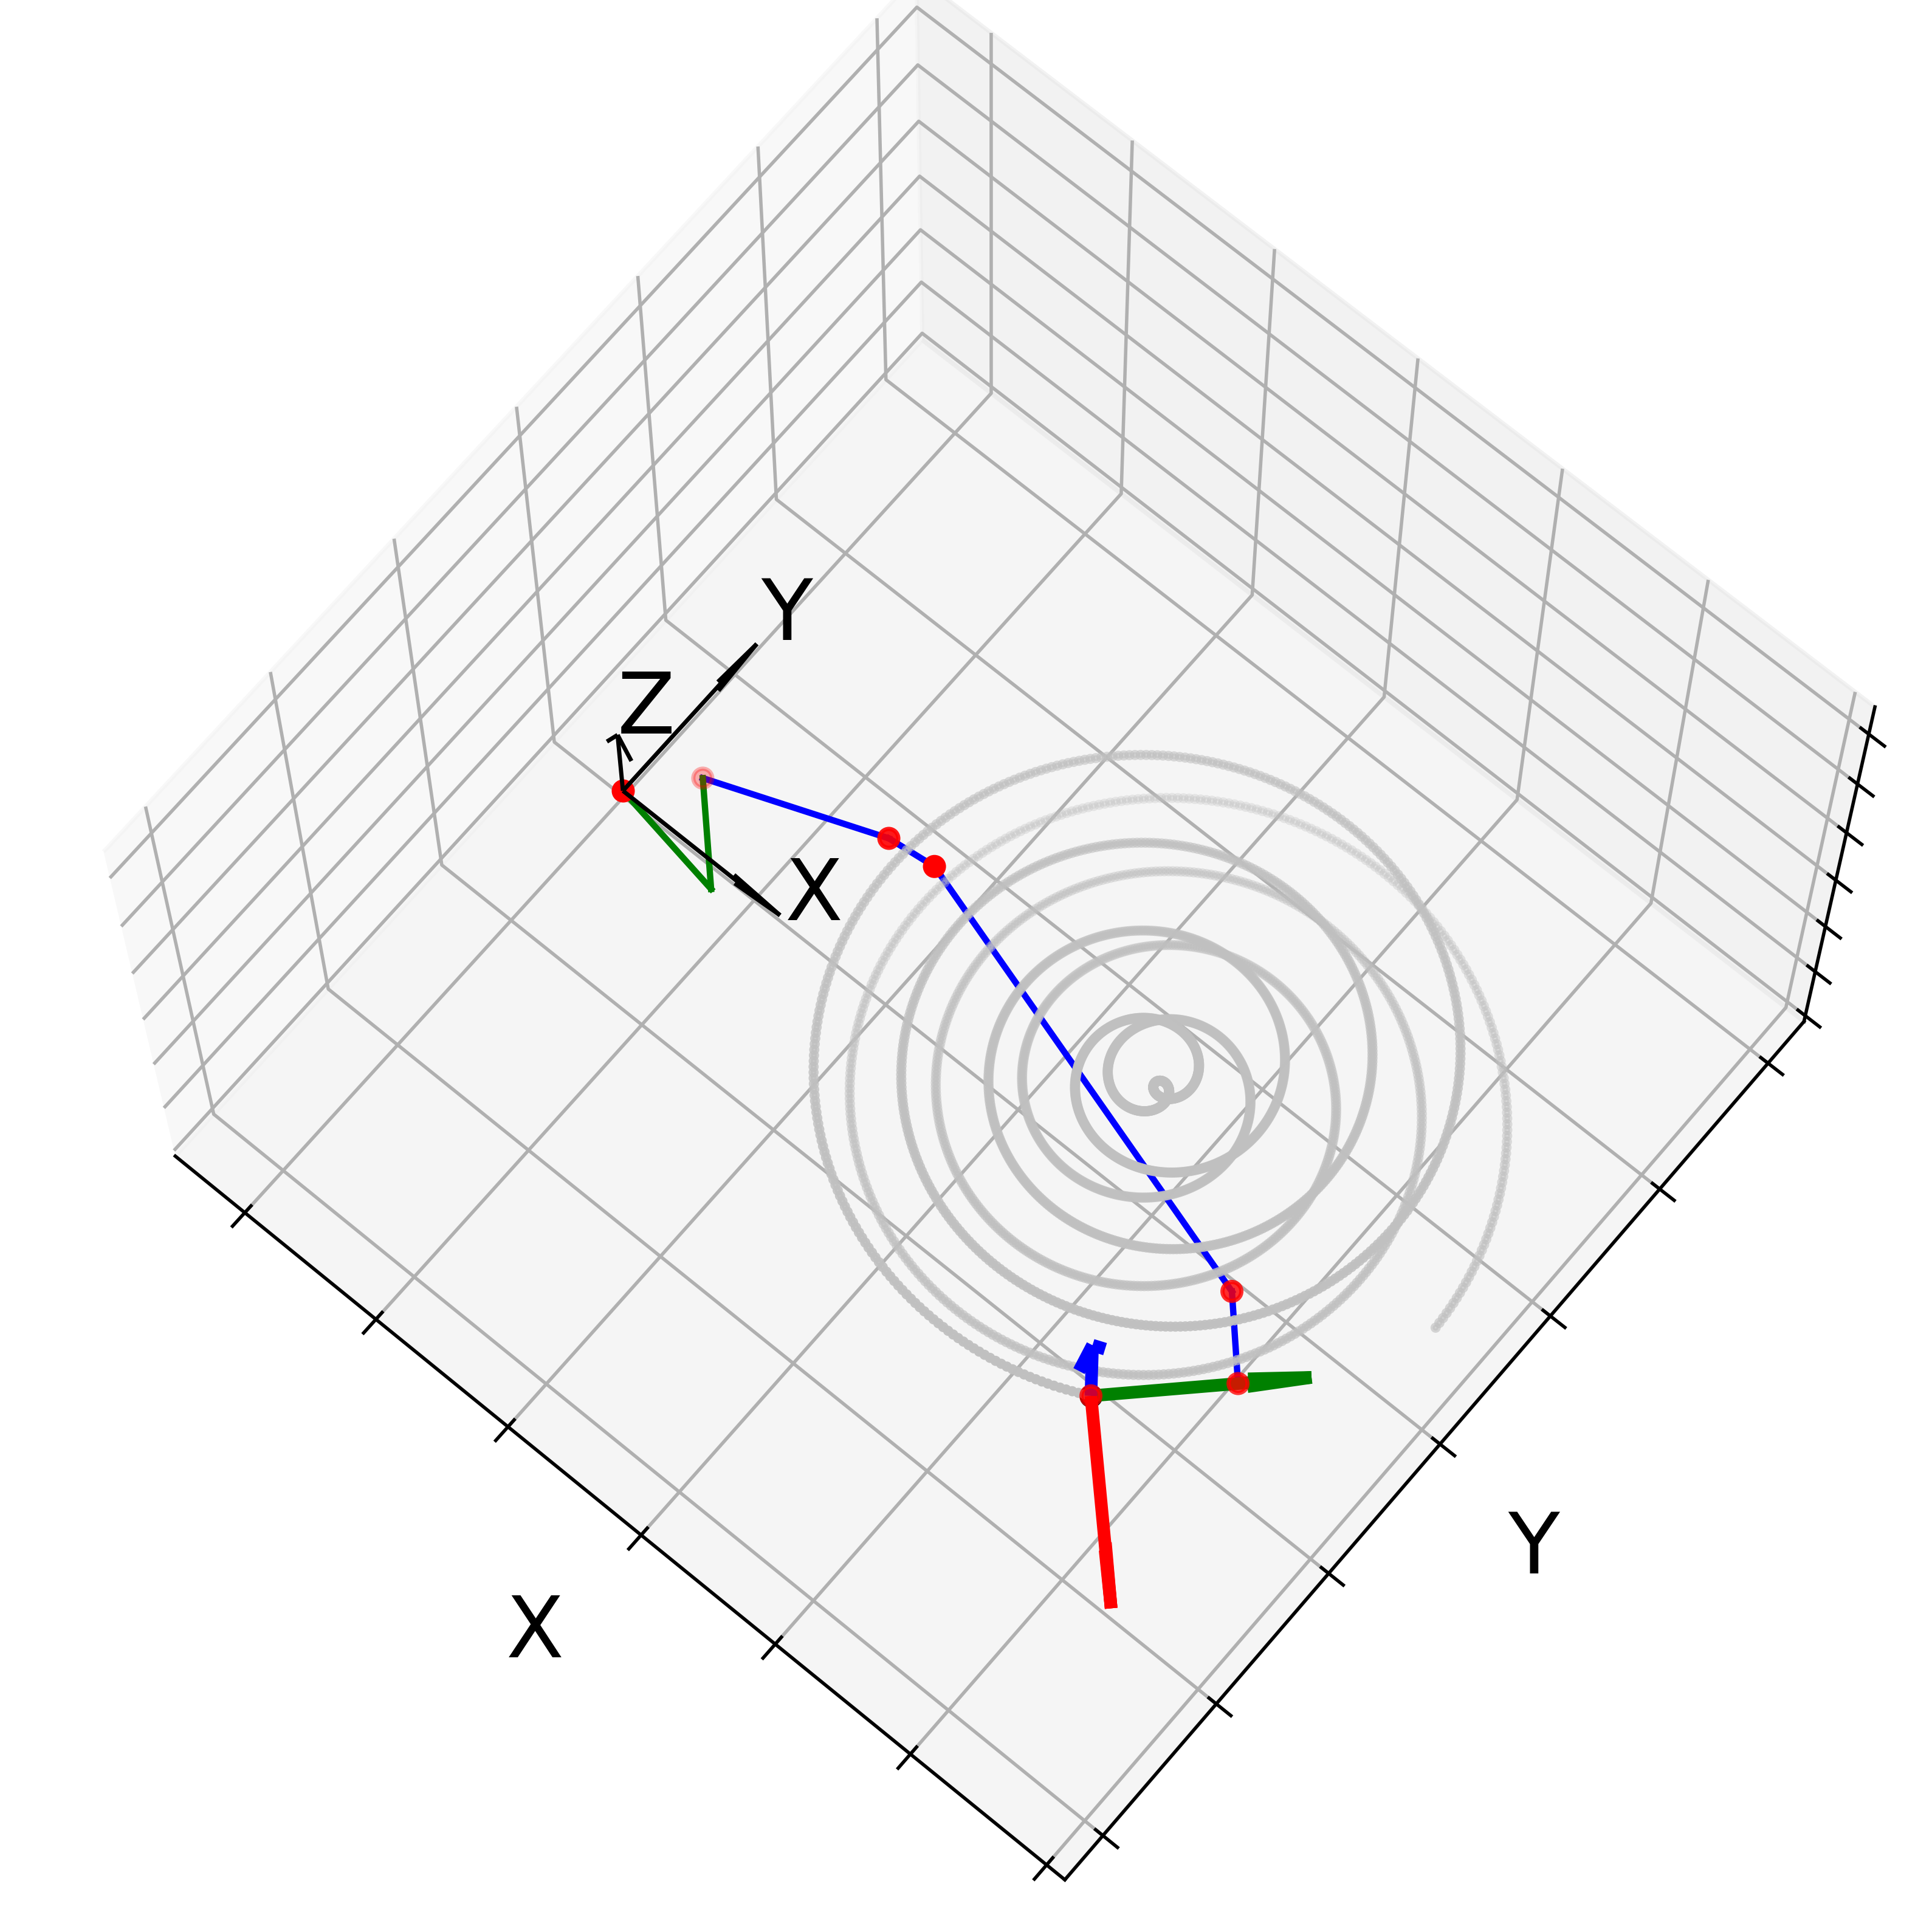
\includegraphics[width=\textwidth]{figures/robotANDpath1_-45.png}
		\caption{Toolpath 1 with A=0, B=0 and C = -45°}
		\label{TP1-25}
	\end{minipage}\hfill
	\begin{minipage}{0.5\textwidth}
		\includegraphics[width=\textwidth]{figures/robotANDpath1_45.png}
		\caption{Toolpath 1 with A=0, B=0 and C = 45}
		\label{TP1+25}
	\end{minipage}\par
\end{figure}

A total of 55 time series of joint positions are generated. The inverse kinematics algorithm takes on average 30 seconds to calculate the joint values for all 3000 coordinates.

The process parameters are extracted and scaled in relation to each other as described in Chapter \ref{LRC}. It is important to note that the selected process parameters are pre-multiplied by -1 because each process parameter should be minimized.

The arrays of the local ratings are multiplied by the weights selected in table \ref{PPbasic}.
Following this, the local scores of each process parameter can be plotted as a one-dimensional graph, as shown in figure \ref{LS1}. %It can be seen that the local scores of the selected process parameters have a significant variation in the range from -15 to 10 degrees.

\begin{figure}[H]
	\centerline{
\includegraphics[width=1\textwidth]{figures/LocalScores_1.png}}
	\caption{Local scores of each process parameter for toolpath 1}
	\label{LS1}
\end{figure}

\newpage
After that, the local scores are summed up to form the global score. The resulting array displayed in figure \ref{GS1}, shows the global score achieved by setting the rotation around the Z-axis relative to all other analyzed values. The green cross indicates the maximum achievable score and its corresponding rotation in comparison to all analyzed boundary conditions.


\begin{figure}[H]
	\centerline{\includegraphics[width=1\textwidth]{figures/best_c_1.png}}
	\caption{Global score for toolpath 1}
	\label{GS1}
\end{figure}
In this case, the best possible achieved score is 92.81 at -135 degrees. This almost perfect score shows that setting the rotation to -135 degrees results in almost the most minimal direction changes,  most minimal total travel and close to most minimal acceleration in joint~1. It is very important to stress that this rating is only in comparison to the other analyzed boundary conditions.
\newpage
The same analysis with the identical process parameters and weights can be performer with toolpath 2 and toolpath 3. The figure \ref{TP2_combi} and figure \ref{TP3_combi} show the global and local scores for every analyzed value of the redundant DoF. In case of toolpath 2 the best score is 93.4 at -115.0 degrees, while at toolpath 3 the best score is 88 at -80 degrees.



\begin{figure}[H]
\centerline{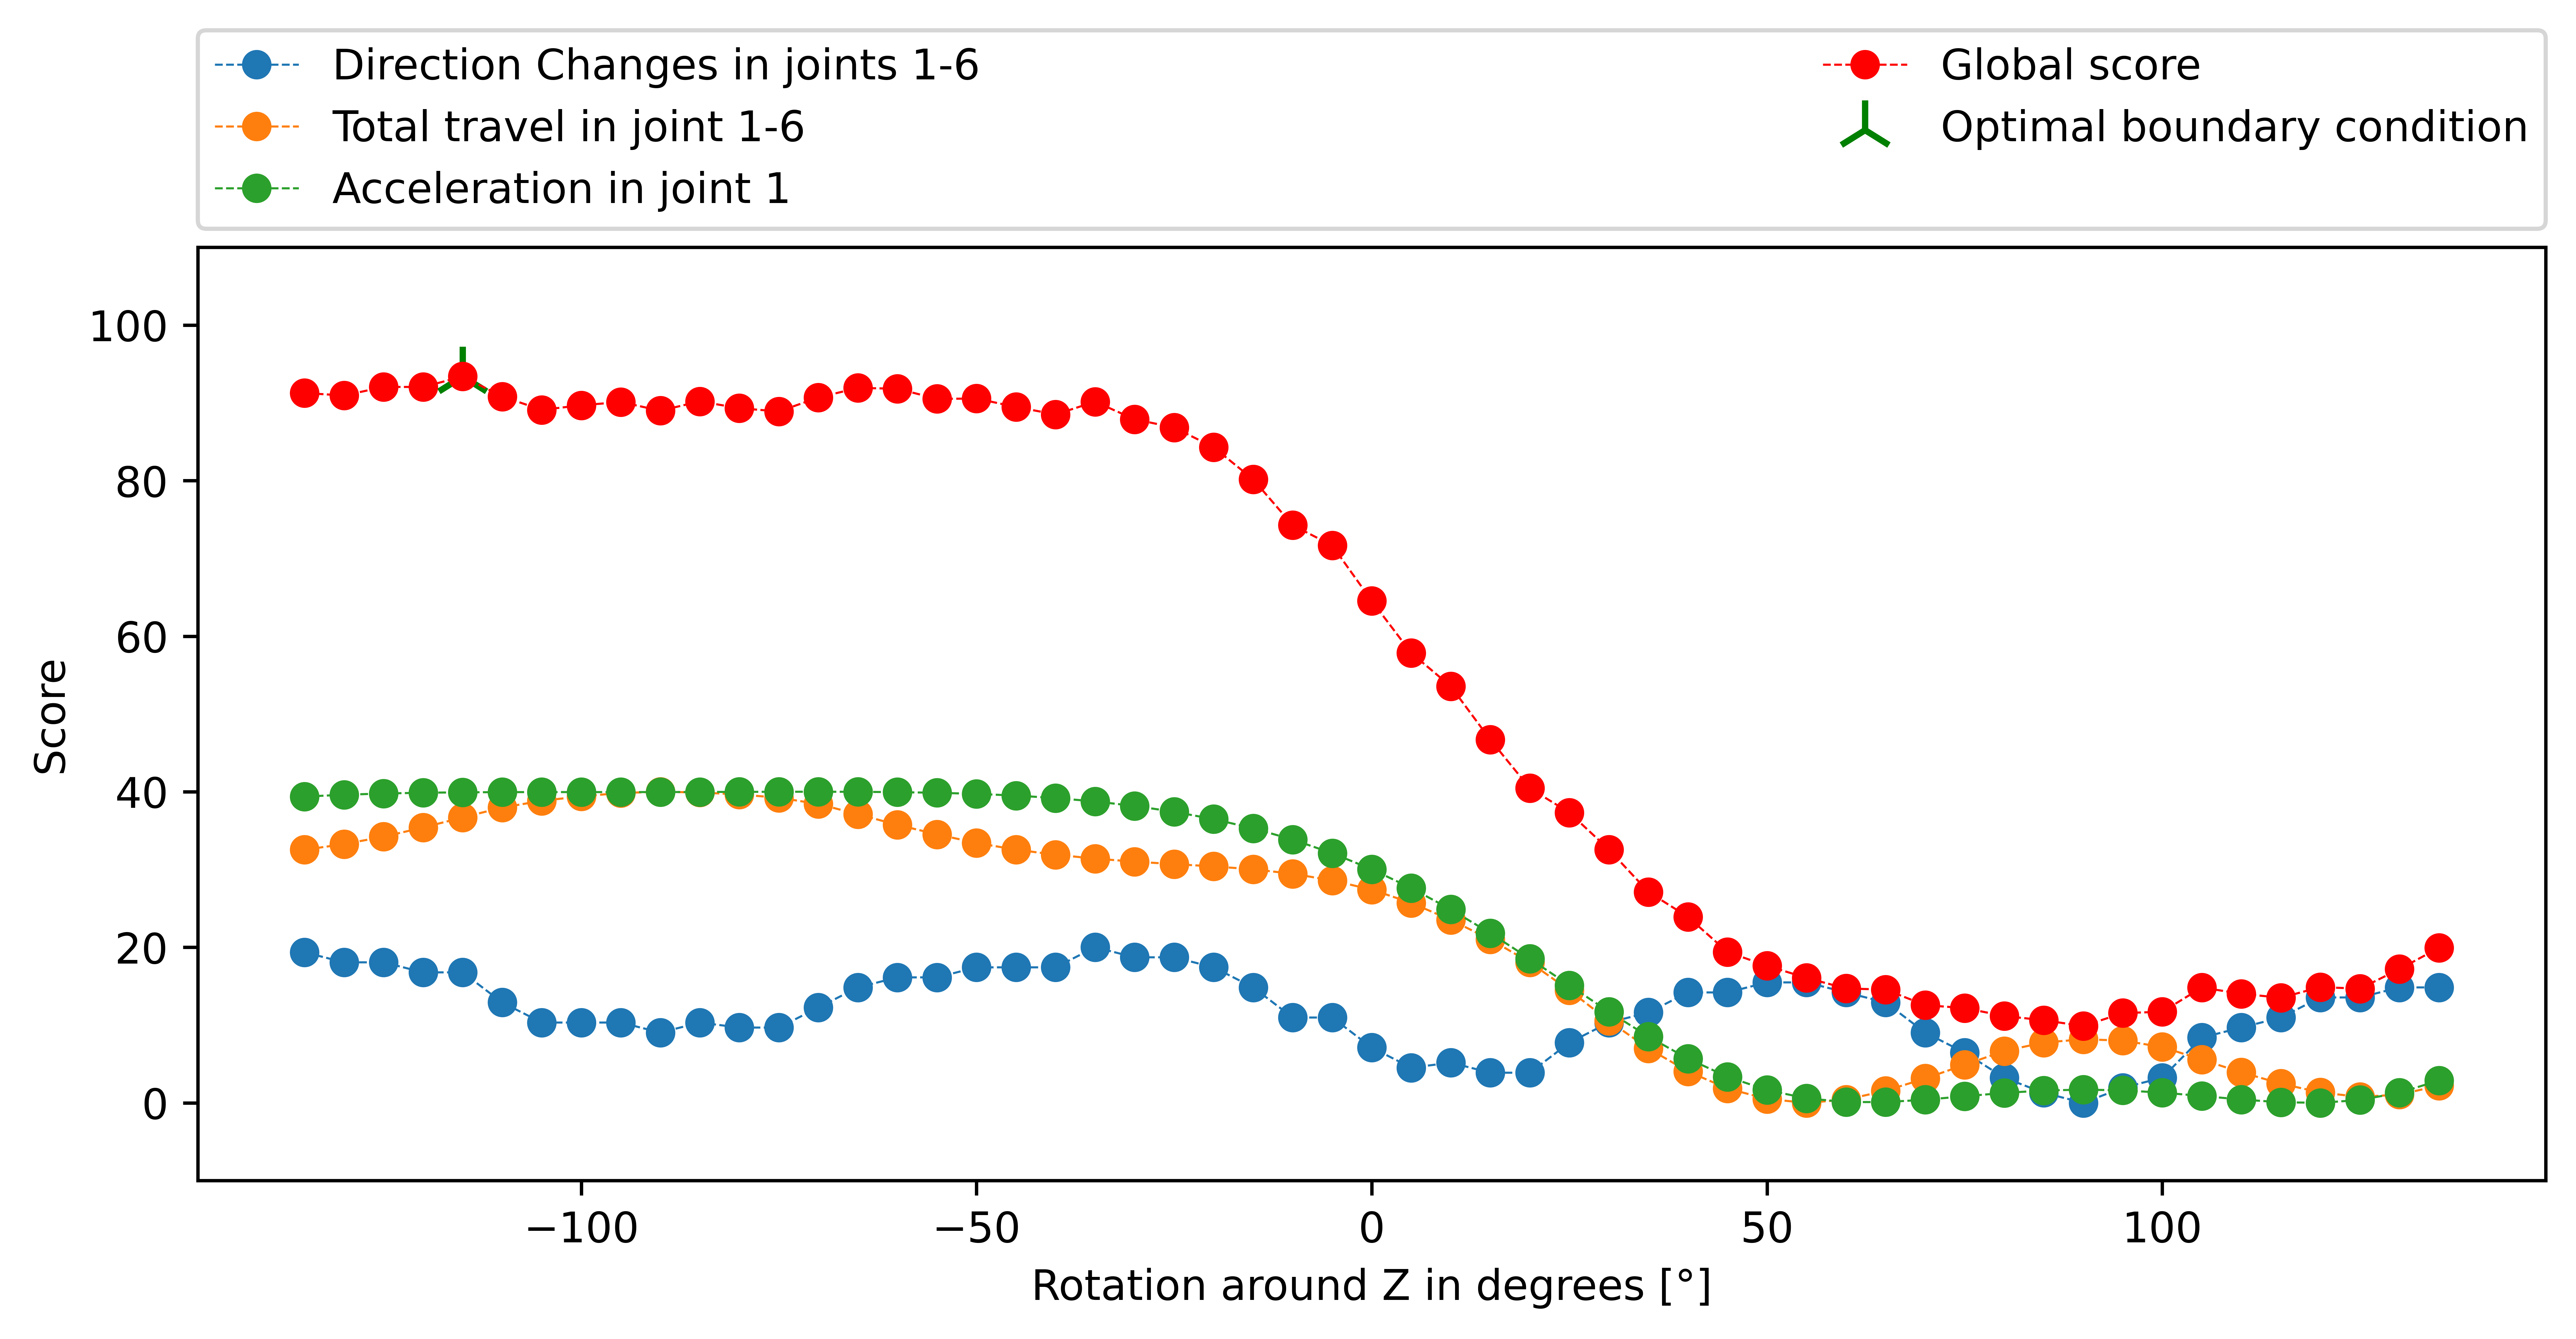
\includegraphics[width=1\textwidth]{figures/best_c_2_combi.png}}
\caption{Global and local scores in toolpath 2 depending on the rotation around Z}
\label{TP2_combi}
\end{figure}
\begin{figure}[H]
\centerline{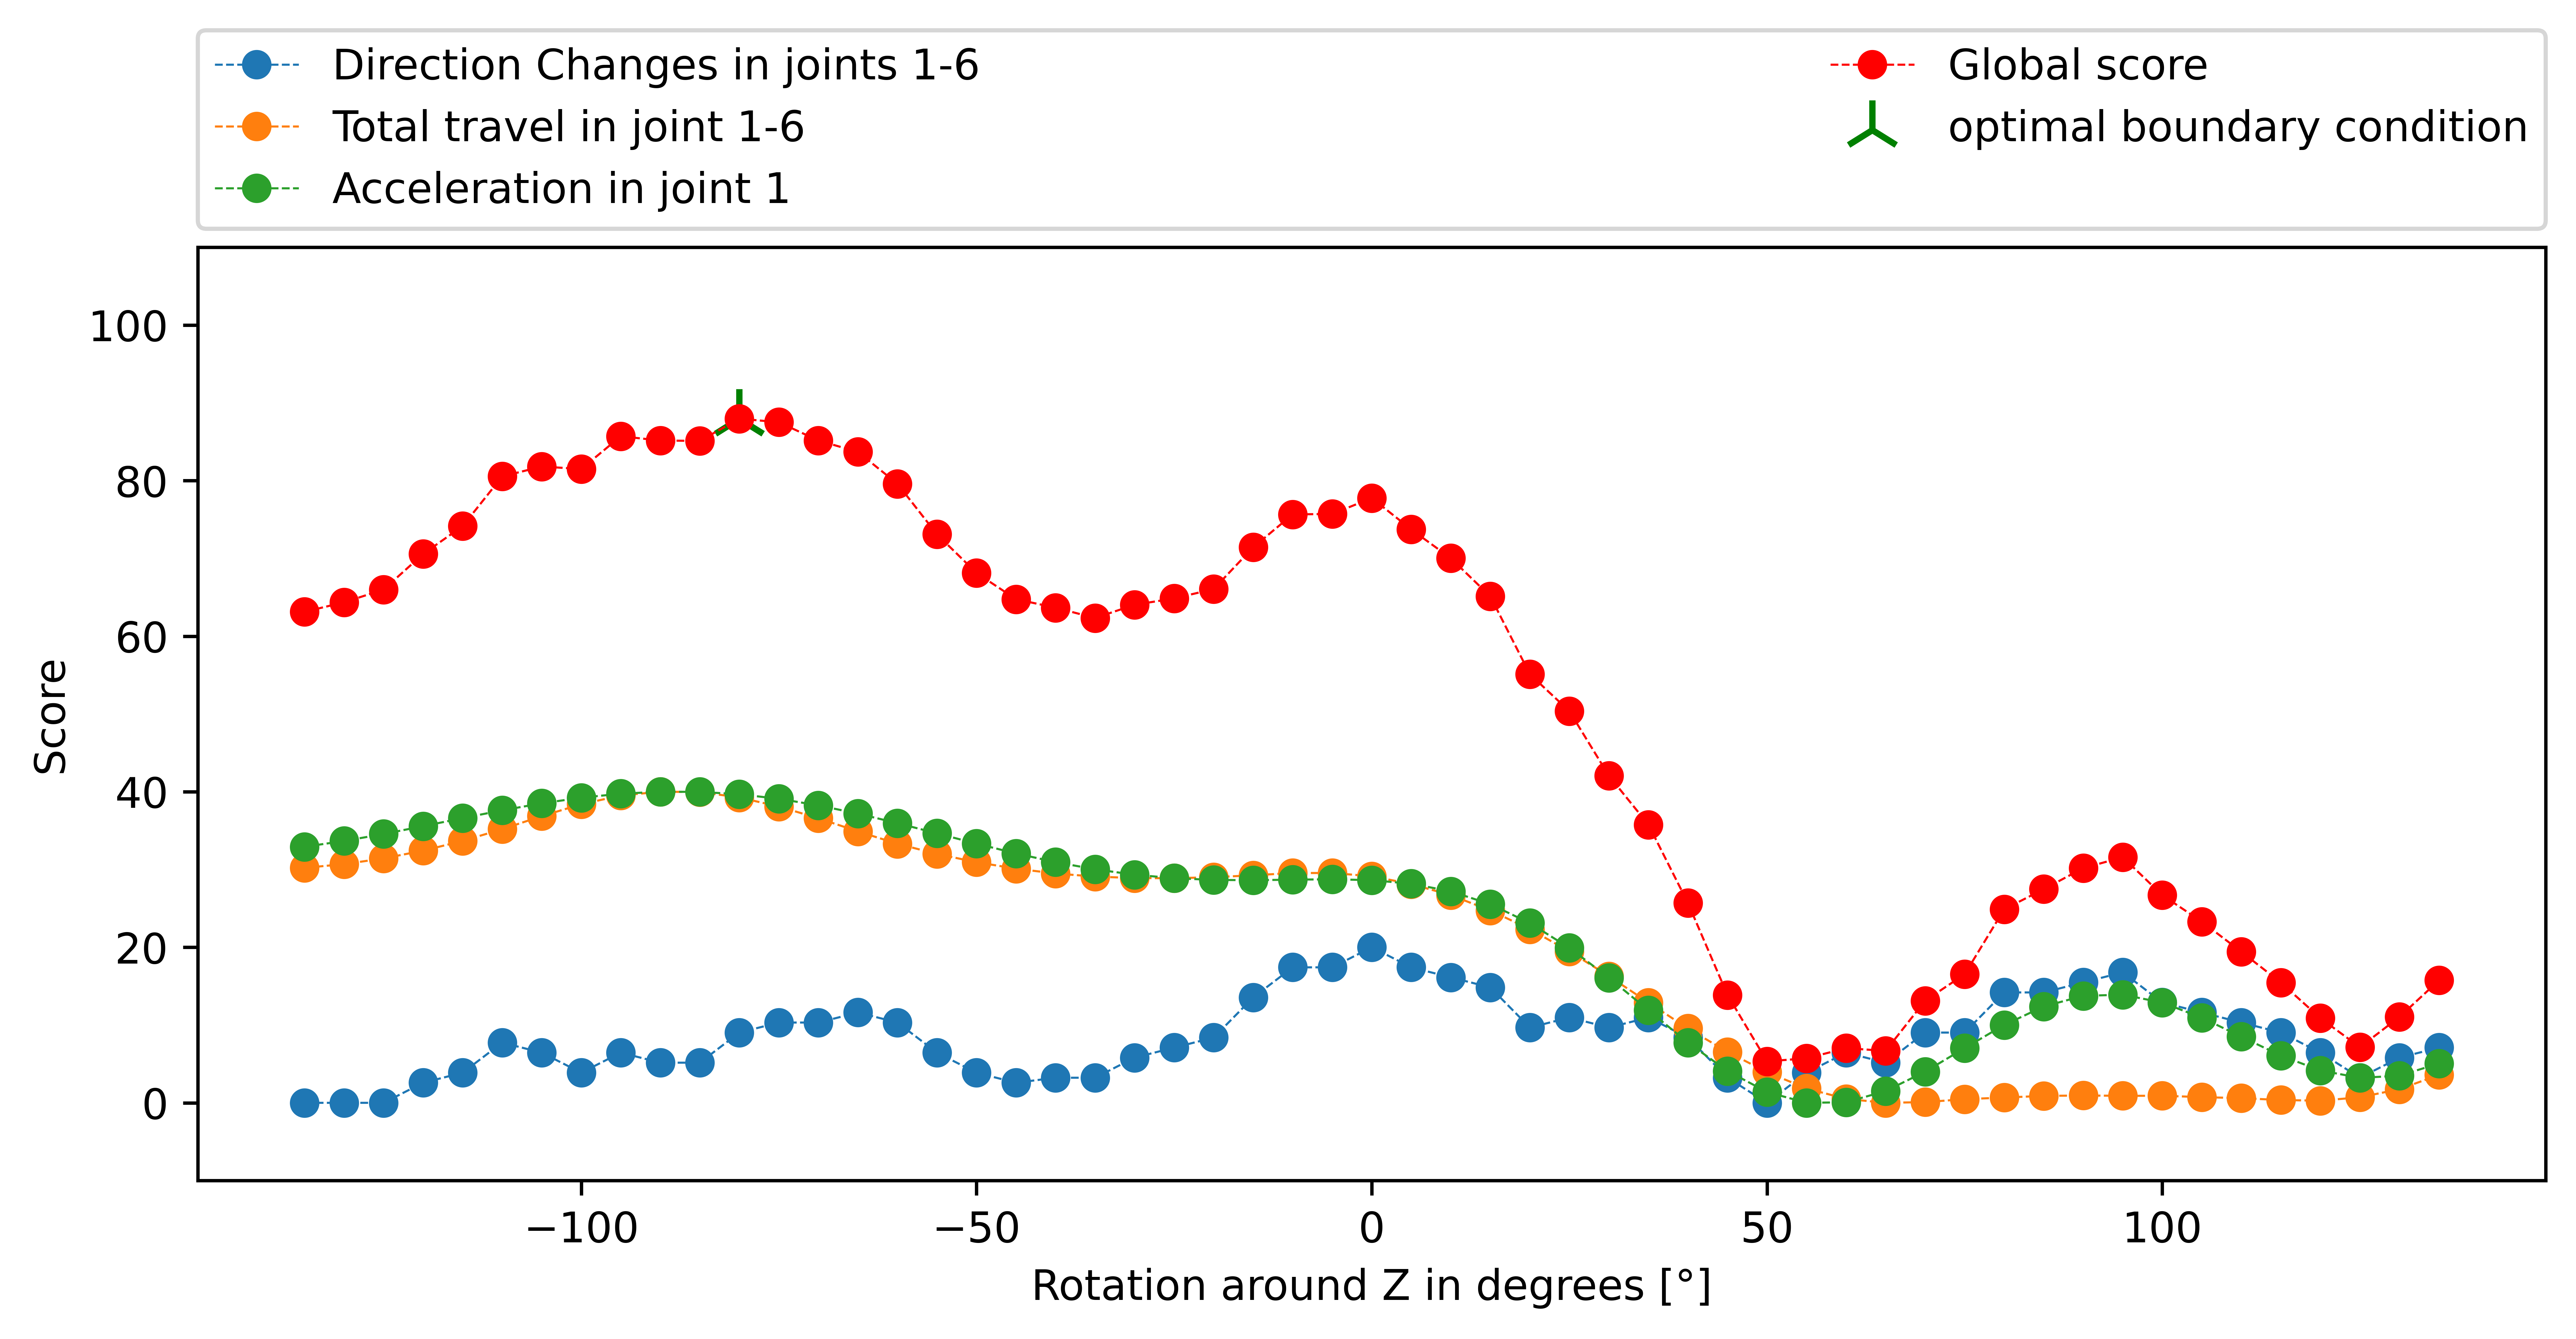
\includegraphics[width=1\textwidth]{figures/best_c_3_combi.png}}
\caption{Global and local scores in toolpath 3 depending on the rotation around Z}
\label{TP3_combi}
\end{figure}
\newpage

\subsection{Toolpath Evaluation with two Redundant DoF}\label{2RDOF}

To add another redundant DoF, a rotary-tilt table is simulated. For now only the tilting is analyzed. All coordinates of the toolpath can be rotated by a set degree around the X-axis. Figure \ref{TP3_0} shows toolpath 3 with no rotation around the X-axis of its coordinate system. Figure \ref{TP3_25} on the other hand shows a rotation of +25 degrees.
\begin{figure}[H]% [H] is so declass\'e!
	\centering
	\begin{minipage}{0.5\textwidth}
		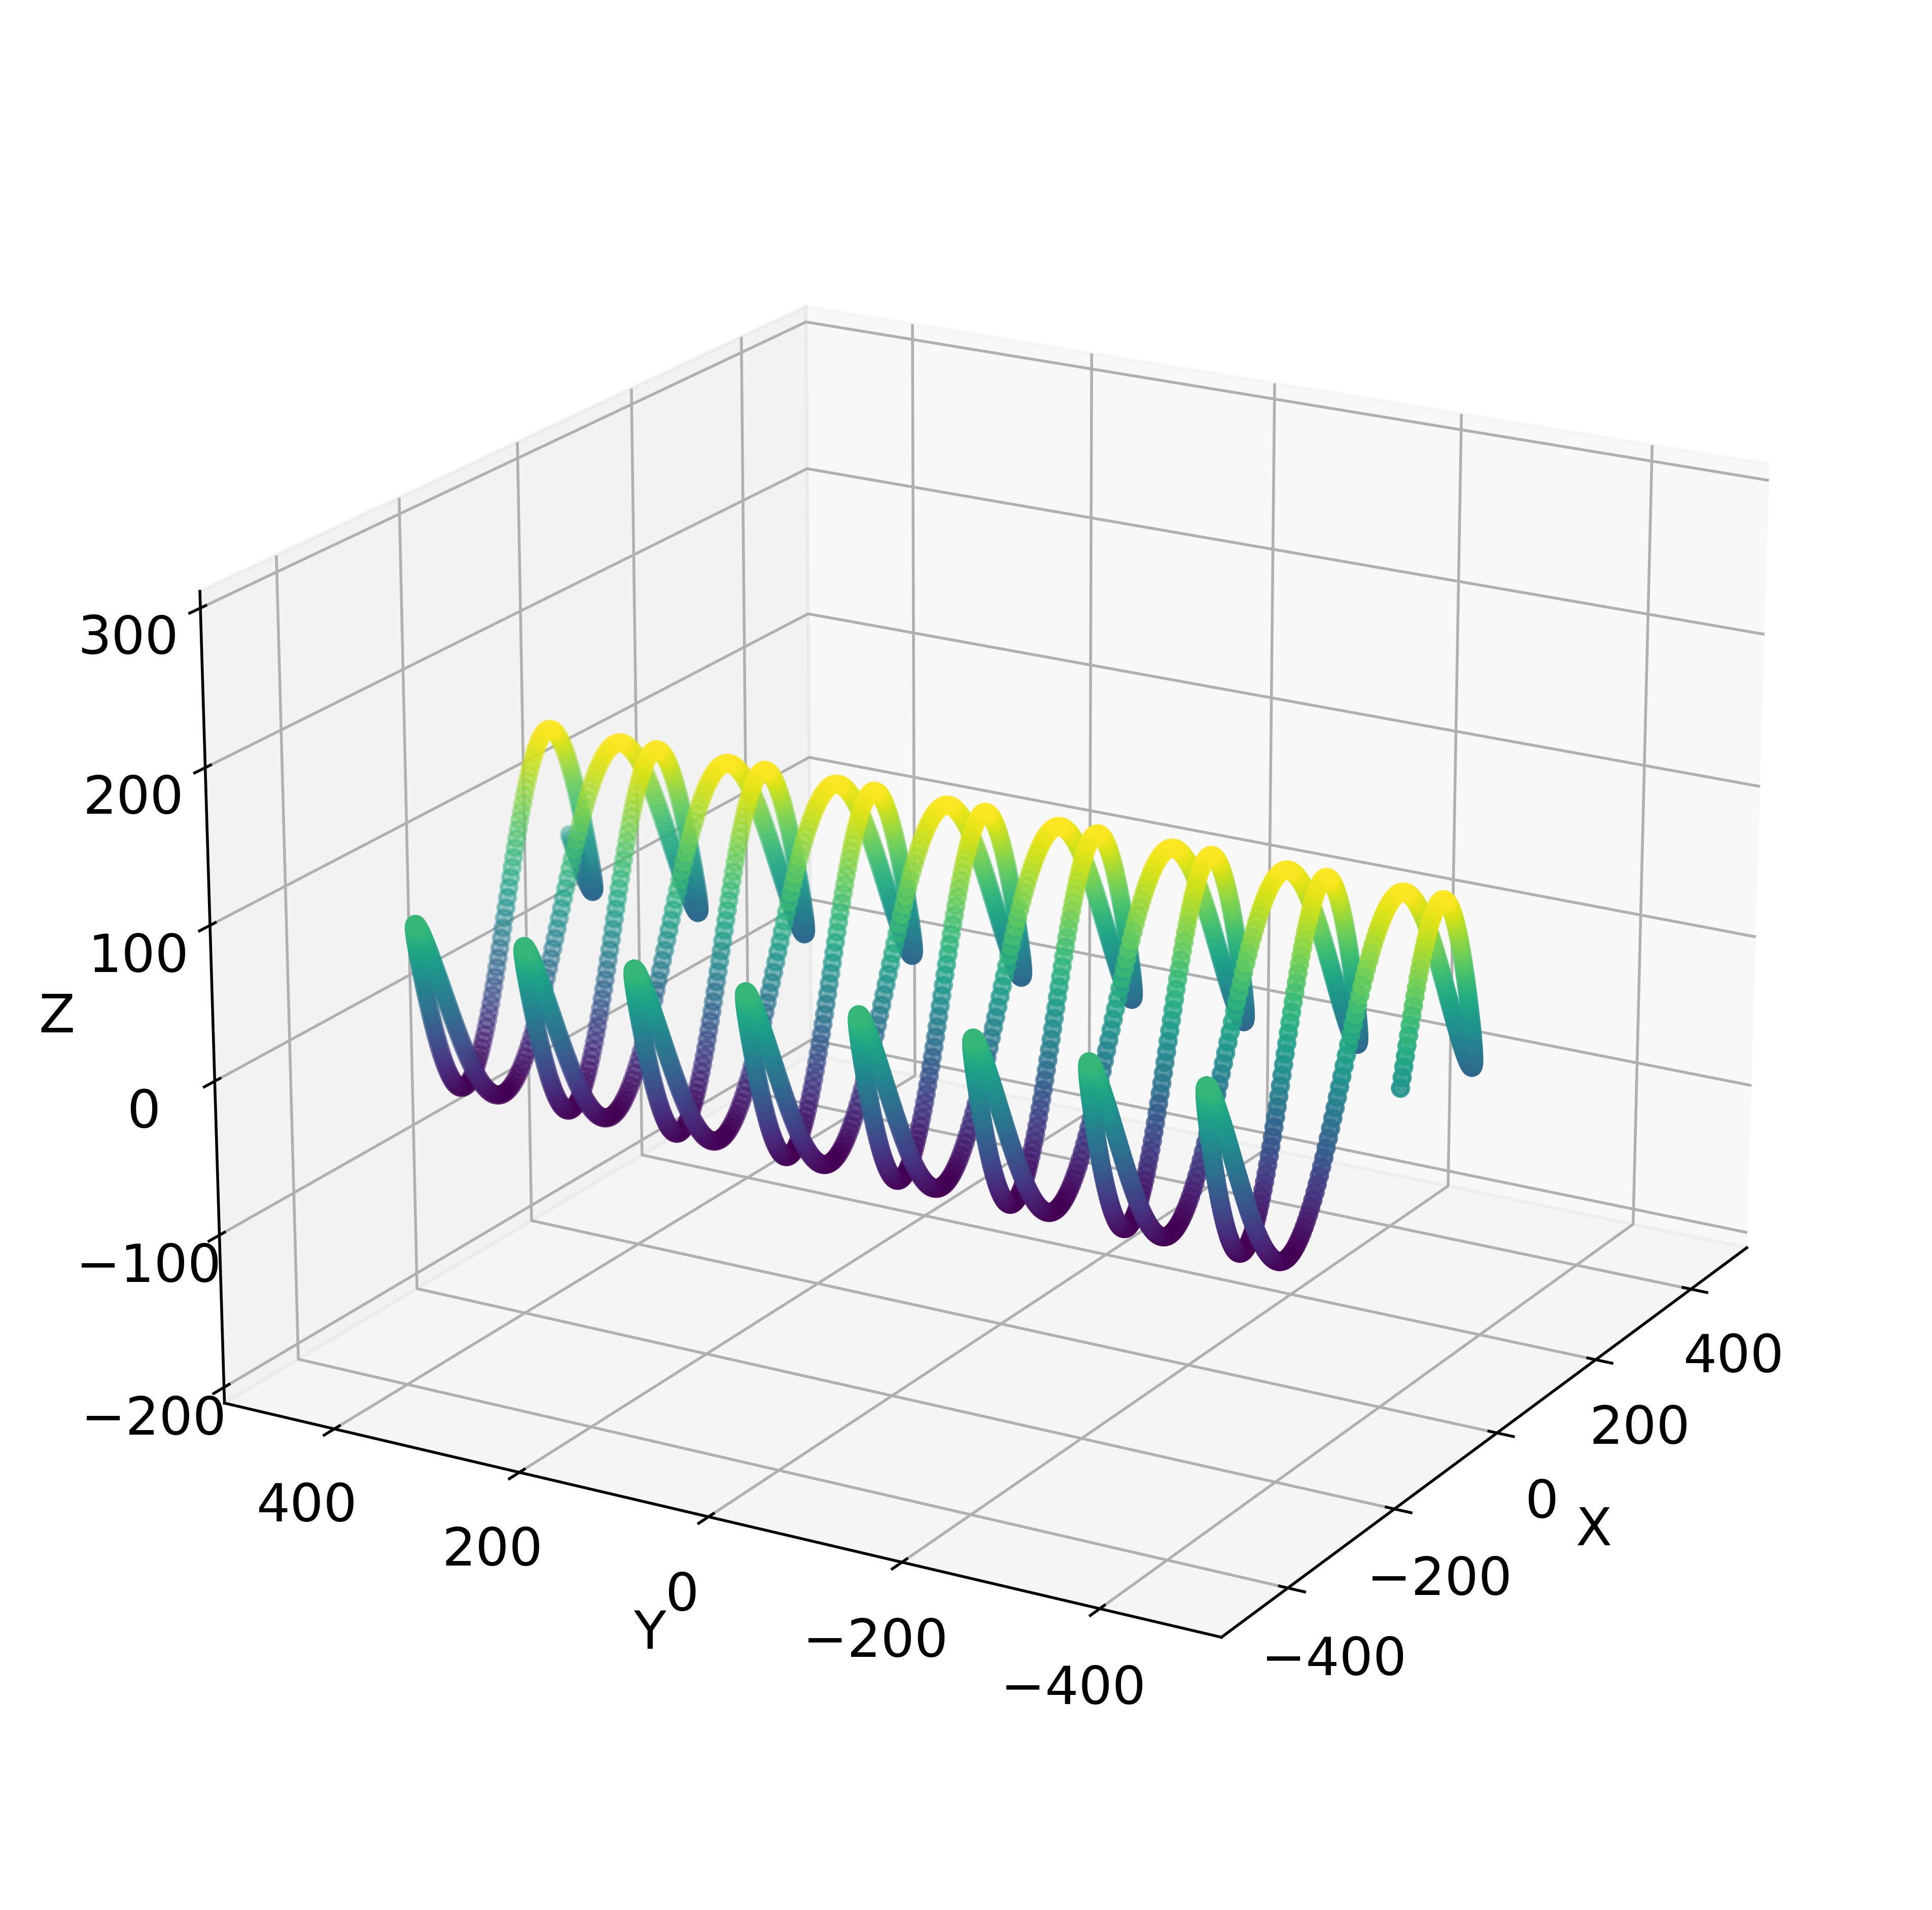
\includegraphics[width=\textwidth]{figures/path3_kipp_0.png}
		\caption{Toolpath 3 with no rotation\newline around the X-axis}
		\label{TP3_0}
	\end{minipage}\hfill
	\begin{minipage}{0.5\textwidth}
		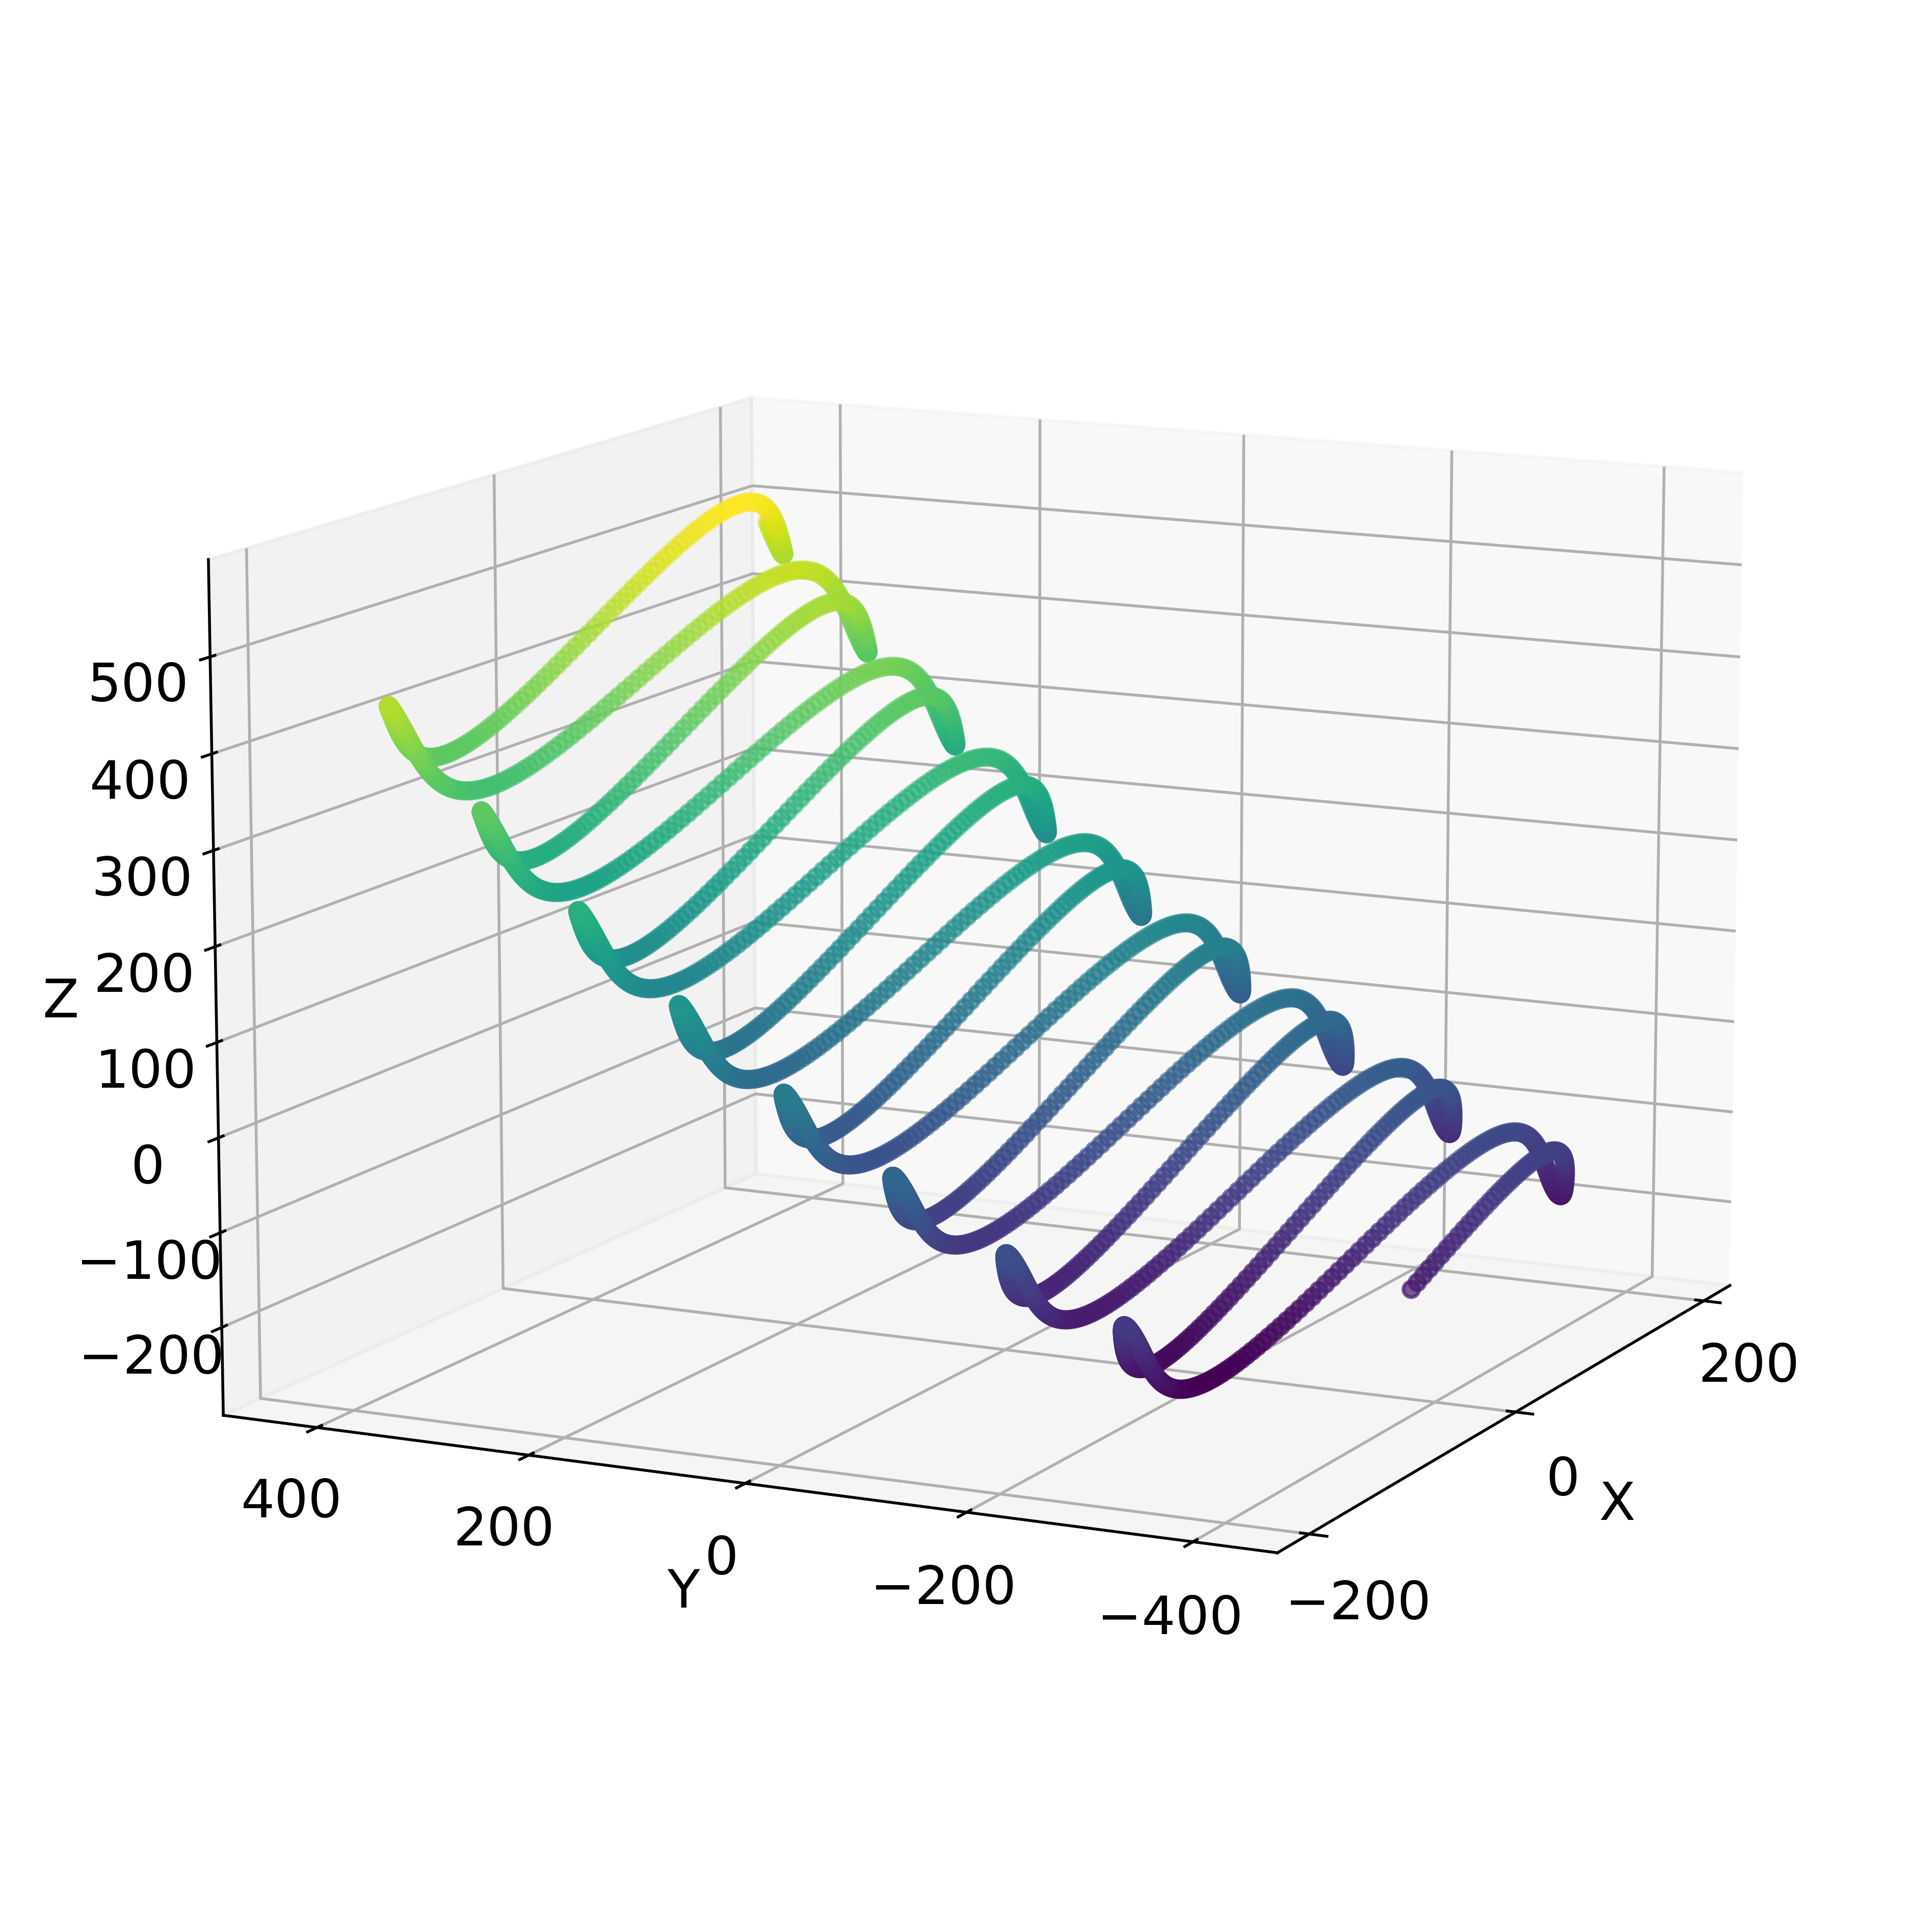
\includegraphics[width=\textwidth]{figures/path3_kipp_25_comparison.png}
		\caption{Toolpath 3 with a rotation\newline of 25 degrees around the X-axis}
		\label{TP3_25}
	\end{minipage}\par
\end{figure}
 

Just as before, for a analysis the same steps need to be performed. The newly selected process parameters are shown in table \ref{PP_2}. All the direction changes of the tilting joints (2+3+5) are summed up as one process parameter and weight with a factor of 0.3. Direction changes in joint 1 and acceleration in joint 4 are selected as individual parameters and are both weight with 0.25. The last parameter is the velocity in joint~6 with a weight of 0.2.  
\begin{table}[H]
	\centering
	\begin{tabular}{||l|l||}
		Process parameters& Importance Factor \\
		\hline
		\hline
		\hline
		Direction changes in joints 2+3+5	&		0.3 \\
		Direction changes in joints 1	&  	0.25 \\
		Acceleration in joint 4	& 		0.25\\
		Velocity in joint 6	& 		0.2\\
		\hline
		\hline
	\end{tabular}
	
	\caption{Selected process parameters and their importance factors for 2 redundant DoF}
	\label{PP_2}
\end{table}



\newpage
Figure \ref{TP3_25_robot} show the robot and its orientation when following the tilted toolpath 3. It is important to note that as the tooolpath is defined in 5 DoF in its own frame, the frame of the TCP also hast to tilt by the same degree as the table. The two redundant DoF in this case are the rotation around the Z-axis in the frame of the tilted toolpath and the tilting of the toolpath itself. This adds another dimension as now 2 parameters can be optimized.


\begin{figure}[H]
	\centerline{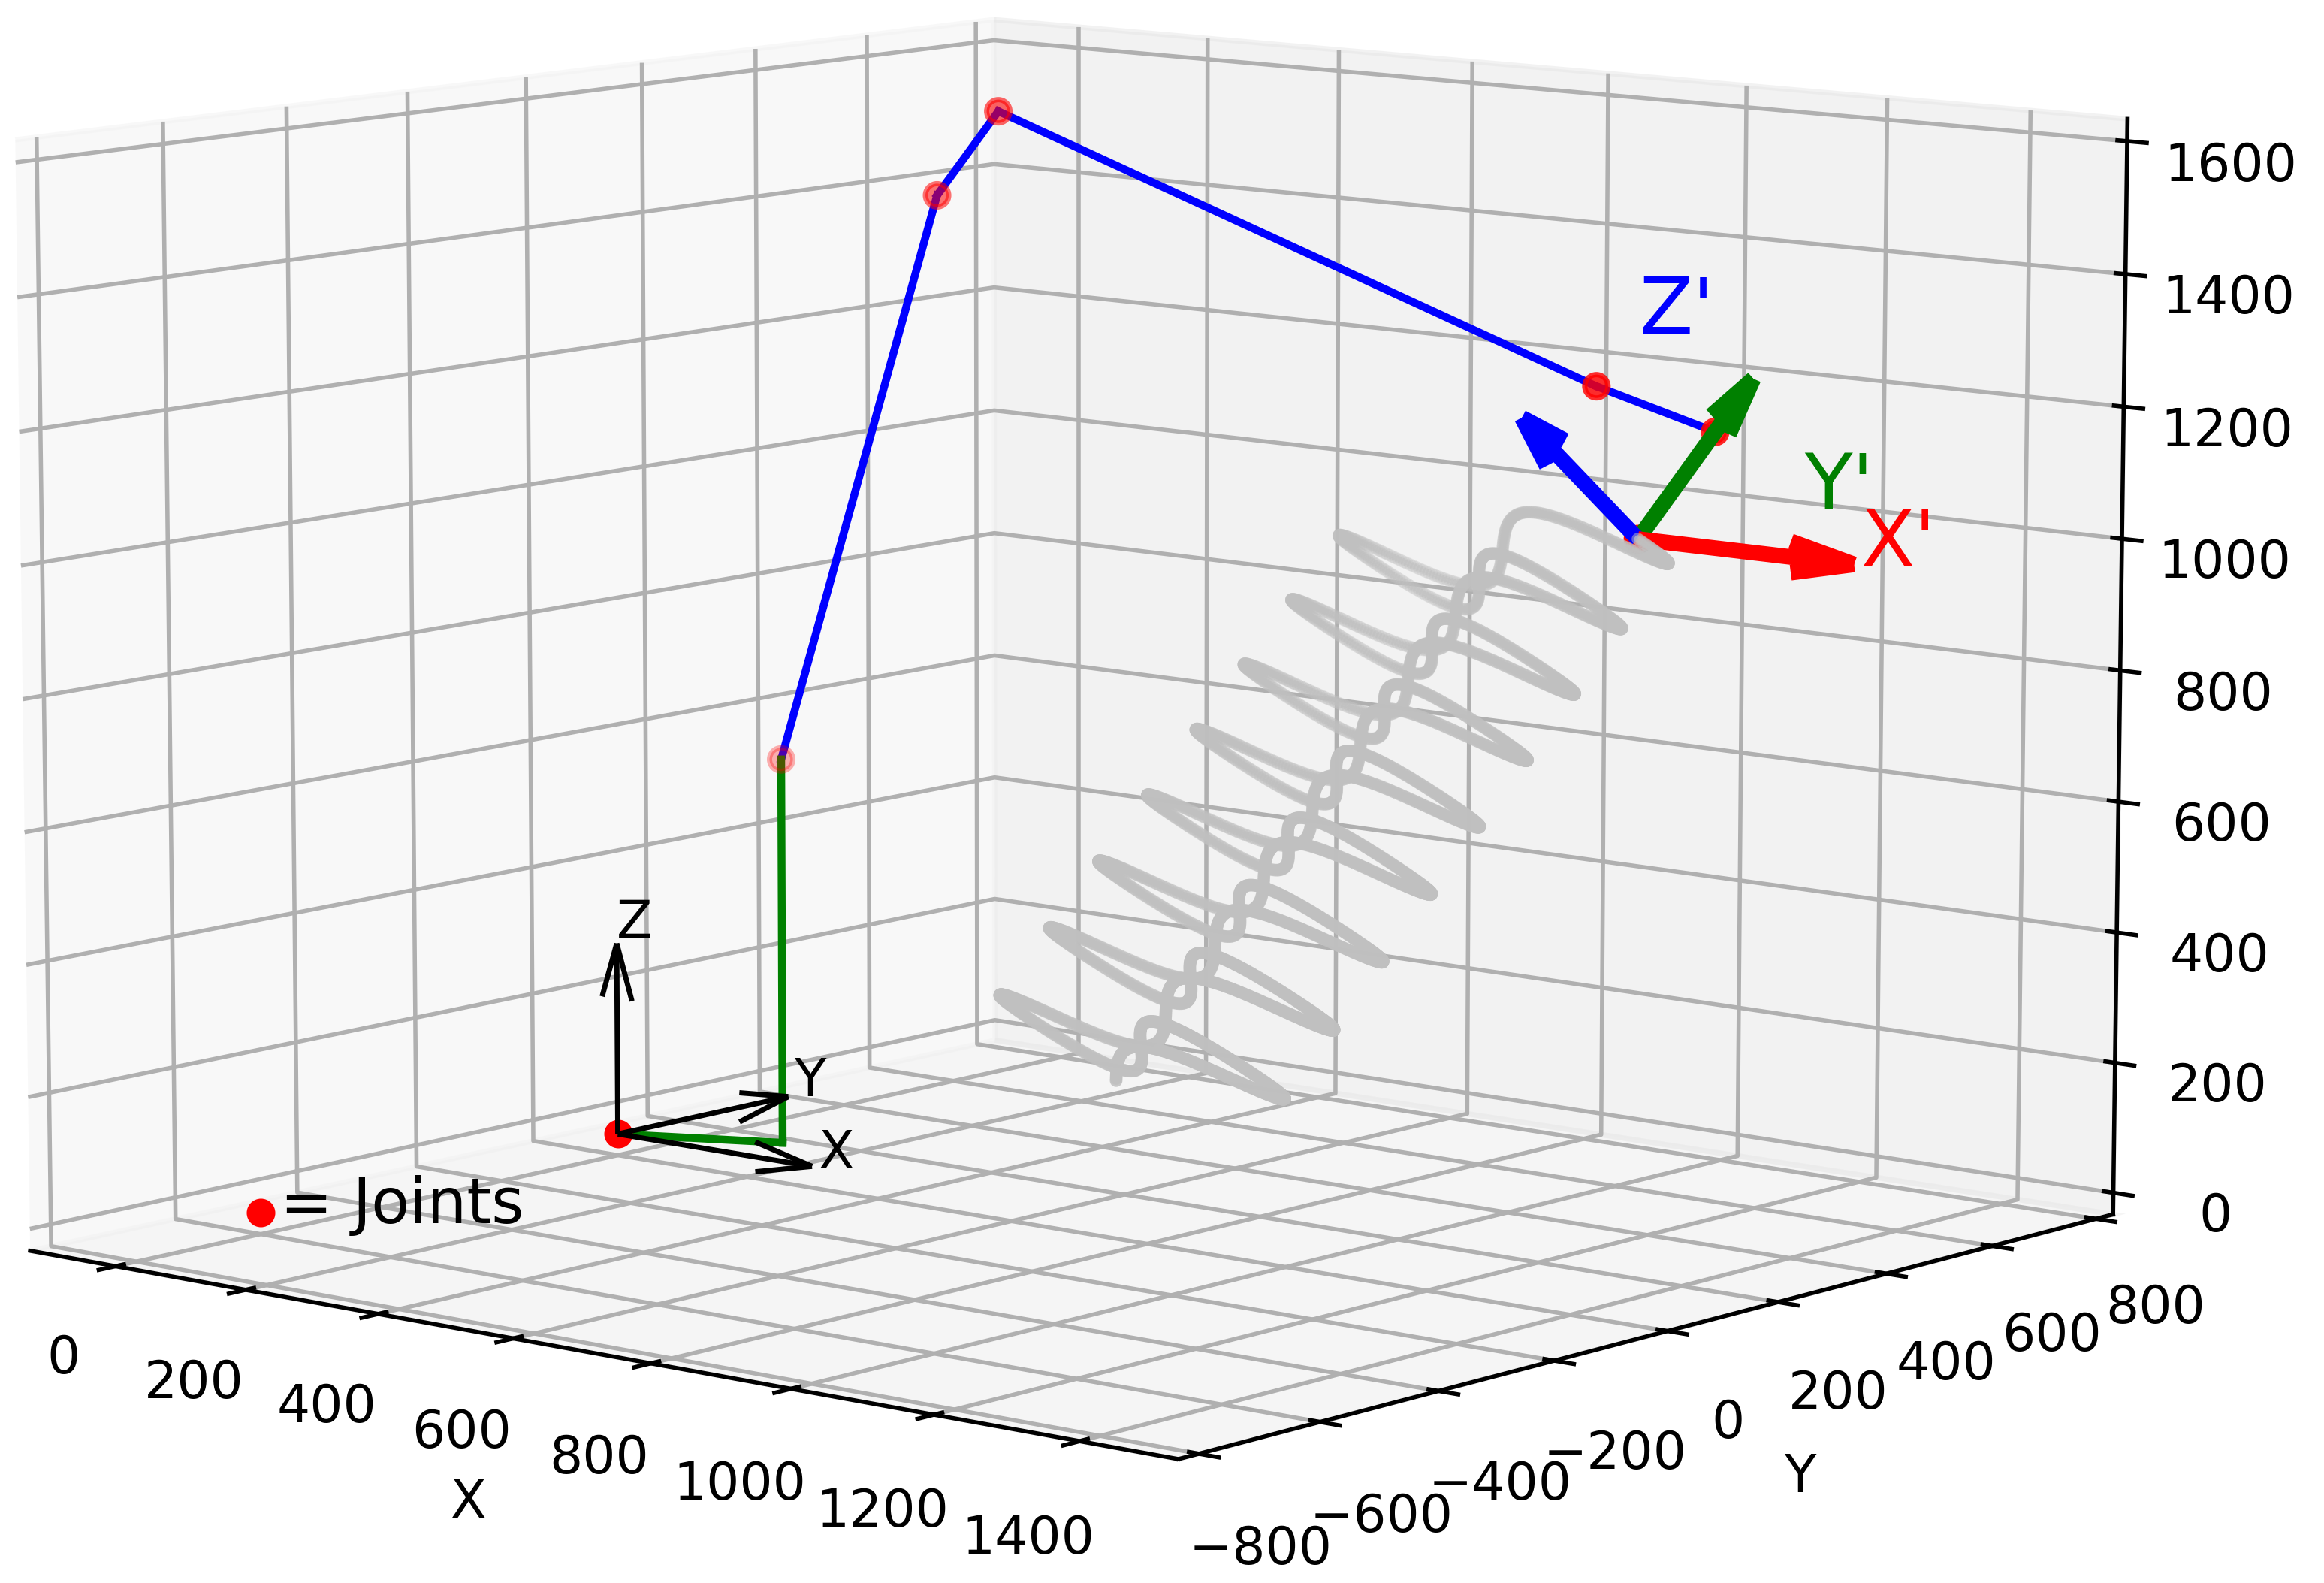
\includegraphics[width=0.9\textwidth]{figures/robotANDpath3_45.png}}
	\caption{Robot following the tilted toolpath 3}
	\label{TP3_25_robot}
\end{figure}

The range of possible tilt positions is ranging from -45° to 45° in 2 degrees increments. 
Now, for every tilt-position and every rotation, the joint angels are generated by inverse kinematics. To save time in computation, only every third coordinate is fed into the inverse kinematic algorithm. This reduces the toolpath by 2000 points and speeds up the calculation. Now it takes only 10 seconds on average to calculate the joint positions. 2530 individual combinations are analyzed.

The extracted process parameters are again multiplied with -1 as the goal is to minimize them. After that the Min-Max scaler is applied. The individual values are summed up and are now represented in form of a matrix. The values of that matrix are visualized in figure~\ref{best_2D}. The maximum achievable score from all possible combinations is 72.96. This score was achieved by setting the tiltig of the table to -3 degrees and the rotation around the Z-axis of the tool to +35 degrees.



\begin{figure}[H]
	\centerline{\includegraphics[width=1\textwidth]{figures/best_2D_3.png}}
	\caption{Hyperplane representing the global score of toolpath 3}
	\label{best_2D}
\end{figure}

\newpage
\subsection{Boundary Condition Optimization }
So far only the analysis of the different boundary condition is performed. For that the defined range of the redundant DoF is explored. After that the best option for the boundary condition can be found. This approach is very time intensive and scales exponentially with additional redundant DoF and finer step size.  

To optimally search this large space and propose the optimal values for the redundant DoF, a PSO-algorithm is proposed. The Individual particles move through the search space by adjusting their positions and velocities based on their own best position and the best position found by the swarm. This cooperation allows the particles to explore the search space more effectively and converge towards the best solution.

The first test is conducted with the with the gobal score matrix of toolpath 3. Initially 20 particles are randomly placed on the plane. Their individual scores are the corresponding global score at their respective position.

In each iteration, the particles update their positions based on their current position, their individual best position and the scores of all other particles. The more particles and more iterations, the more densely the search space can be analyzed. 
Figure \ref{PSO_1}

\begin{figure}[H]
	\centerline{\includegraphics[width=0.8\textwidth]{figures/swarm/3_1.png}}
	\caption{Distributed of particles after the first iteration}
	\label{PSO_1}
\end{figure}



Figures \ref{2} to \ref{5} show how the particles converge to the found maximum. This convergence takes place in 5 iterations. The best position of all 5 particles is equal to the global maximum as mentioned in Chapter \ref{2RDOF}. This example shows that it is generally possible to search a high dimensional space without the necessity to compute all possible combinations.


\begin{figure}[H]
	\centering
	\begin{minipage}{0.5\textwidth}
		\includegraphics[width=\textwidth]{figures/swarm/3_2.png}
		\caption{PSO Iteration 2}
		\label{2}
	\end{minipage}\hfill
	\begin{minipage}{0.5\textwidth}
		\includegraphics[width=\textwidth]{figures/swarm/3_3.png}
		\caption{PSO Iteration 3}
		\label{3}
	\end{minipage}\par
\end{figure}	
\begin{figure}[H]	
		\centering
	\begin{minipage}{0.5\textwidth}
		\includegraphics[width=\textwidth]{figures/swarm/3_4.png}
		\caption{PSO Iteration 4}
		\label{4}
	\end{minipage}\hfill
	\begin{minipage}{0.5\textwidth}
		\includegraphics[width=\textwidth]{figures/swarm/3_5.png}
		\caption{PSO Iteration 5}
		\label{5}
	\end{minipage}\par
\end{figure}

One important factor in this test is that the scores are already calculated. The global score matrix is calculated relative to all possible combinations of the different boundary conditions. However, in the intended scenario where this method is used to find the optimal boundary condition, such a matrix does not exist.

Therefore, the scores of the individual positions have to be compared relative to each other at each iteration, taking into consideration the past iterations. This method is shown in Figure \ref{swarmloop}. Initially, a set number of particles is randomly placed on the plane, with the X and Y values defining the selected boundary conditions. For each selected boundary condition, the joint angles are calculated using the inverse kinematic approach. After that, the analyzed process parameters are extracted and the joint angles are stored. The score for each current position is calculated relative to all stored toolpaths.

It is possible that a particle once had a position with a very high score compared to the other available toolpaths at that time. Therefore, after each iteration, it is necessary to update the score of the most optimal position of the particle as more boundary conditions are analyzed. This is done to ensure that an initially relative score, which may have been mistakenly selected as the best, does not influence the subsequent search directions.

\begin{figure}[H]
	\centerline{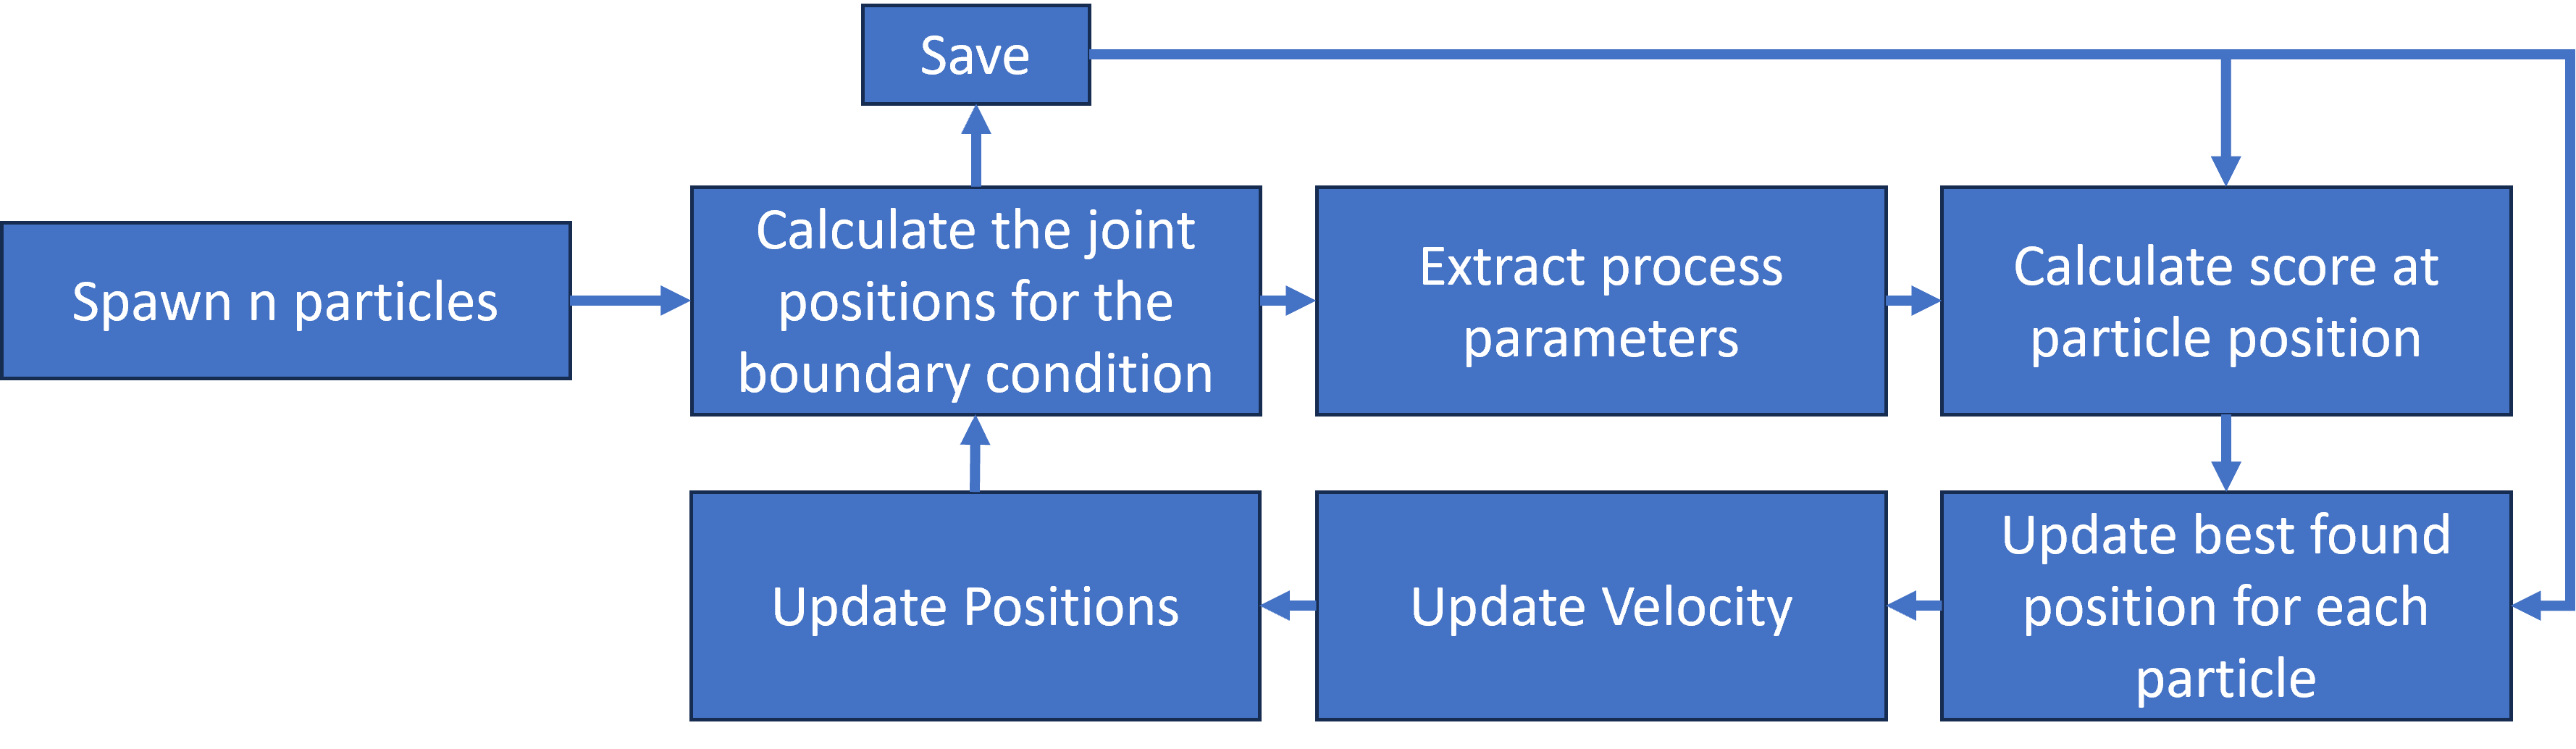
\includegraphics[width=0.9\textwidth]{figures/swarmloop.png}}
	\caption{PSO-Loop}
	\label{swarmloop}
\end{figure}

Following this approach, the following results are calculated. It is important to note that the underlying colors from the global score matrix are not available to the PSO algorithm. They are only used to evaluate the behavior of the particles.

Figures \ref{1_true} to \ref{4_true} show the progression of the individual particles. The green circle indicates the overall best position found by the particles so far.

\begin{figure}[H]
	\centering
	\begin{minipage}{0.5\textwidth}
		\includegraphics[width=\textwidth]{figures/swarm_true/3_1.png}
		\caption{PSO Iteration 1}
		\label{1_true}
	\end{minipage}\hfill
	\begin{minipage}{0.5\textwidth}
		\includegraphics[width=\textwidth]{figures/swarm_true/3_2.png}
		\caption{PSO Iteration 2}
		\label{2_true}
	\end{minipage}\par
\end{figure}	

\begin{figure}[H]	
	\centering
	\begin{minipage}{0.5\textwidth}
		\includegraphics[width=\textwidth]{figures/swarm_true/3_3.png}
		\caption{PSO Iteration 3}
		\label{3_true}
	\end{minipage}\hfill
	\begin{minipage}{0.5\textwidth}
		\includegraphics[width=\textwidth]{figures/swarm_true/3_4.png}
		\caption{PSO Iteration 4}
		\label{4_true}
	\end{minipage}\par
\end{figure}

Figure \ref{5_true} shows the position of the particles after the final fifth iteration.

\begin{figure}[H]
	\centerline{\includegraphics[width=0.9\textwidth]{figures/swarm_true/3_5.png}}
	\caption{PSO iteration 5}
	\label{5_true}
\end{figure}

Figures \ref{5_true_1} and \ref{5_true_2} show the final position of the particles when the first and second toolpath is analyzed, respectively. In both cases the PSO-algorithm succeeded to find the globally optimal condition.
\begin{figure}[H]	
	\centering
	\begin{minipage}{0.5\textwidth}
		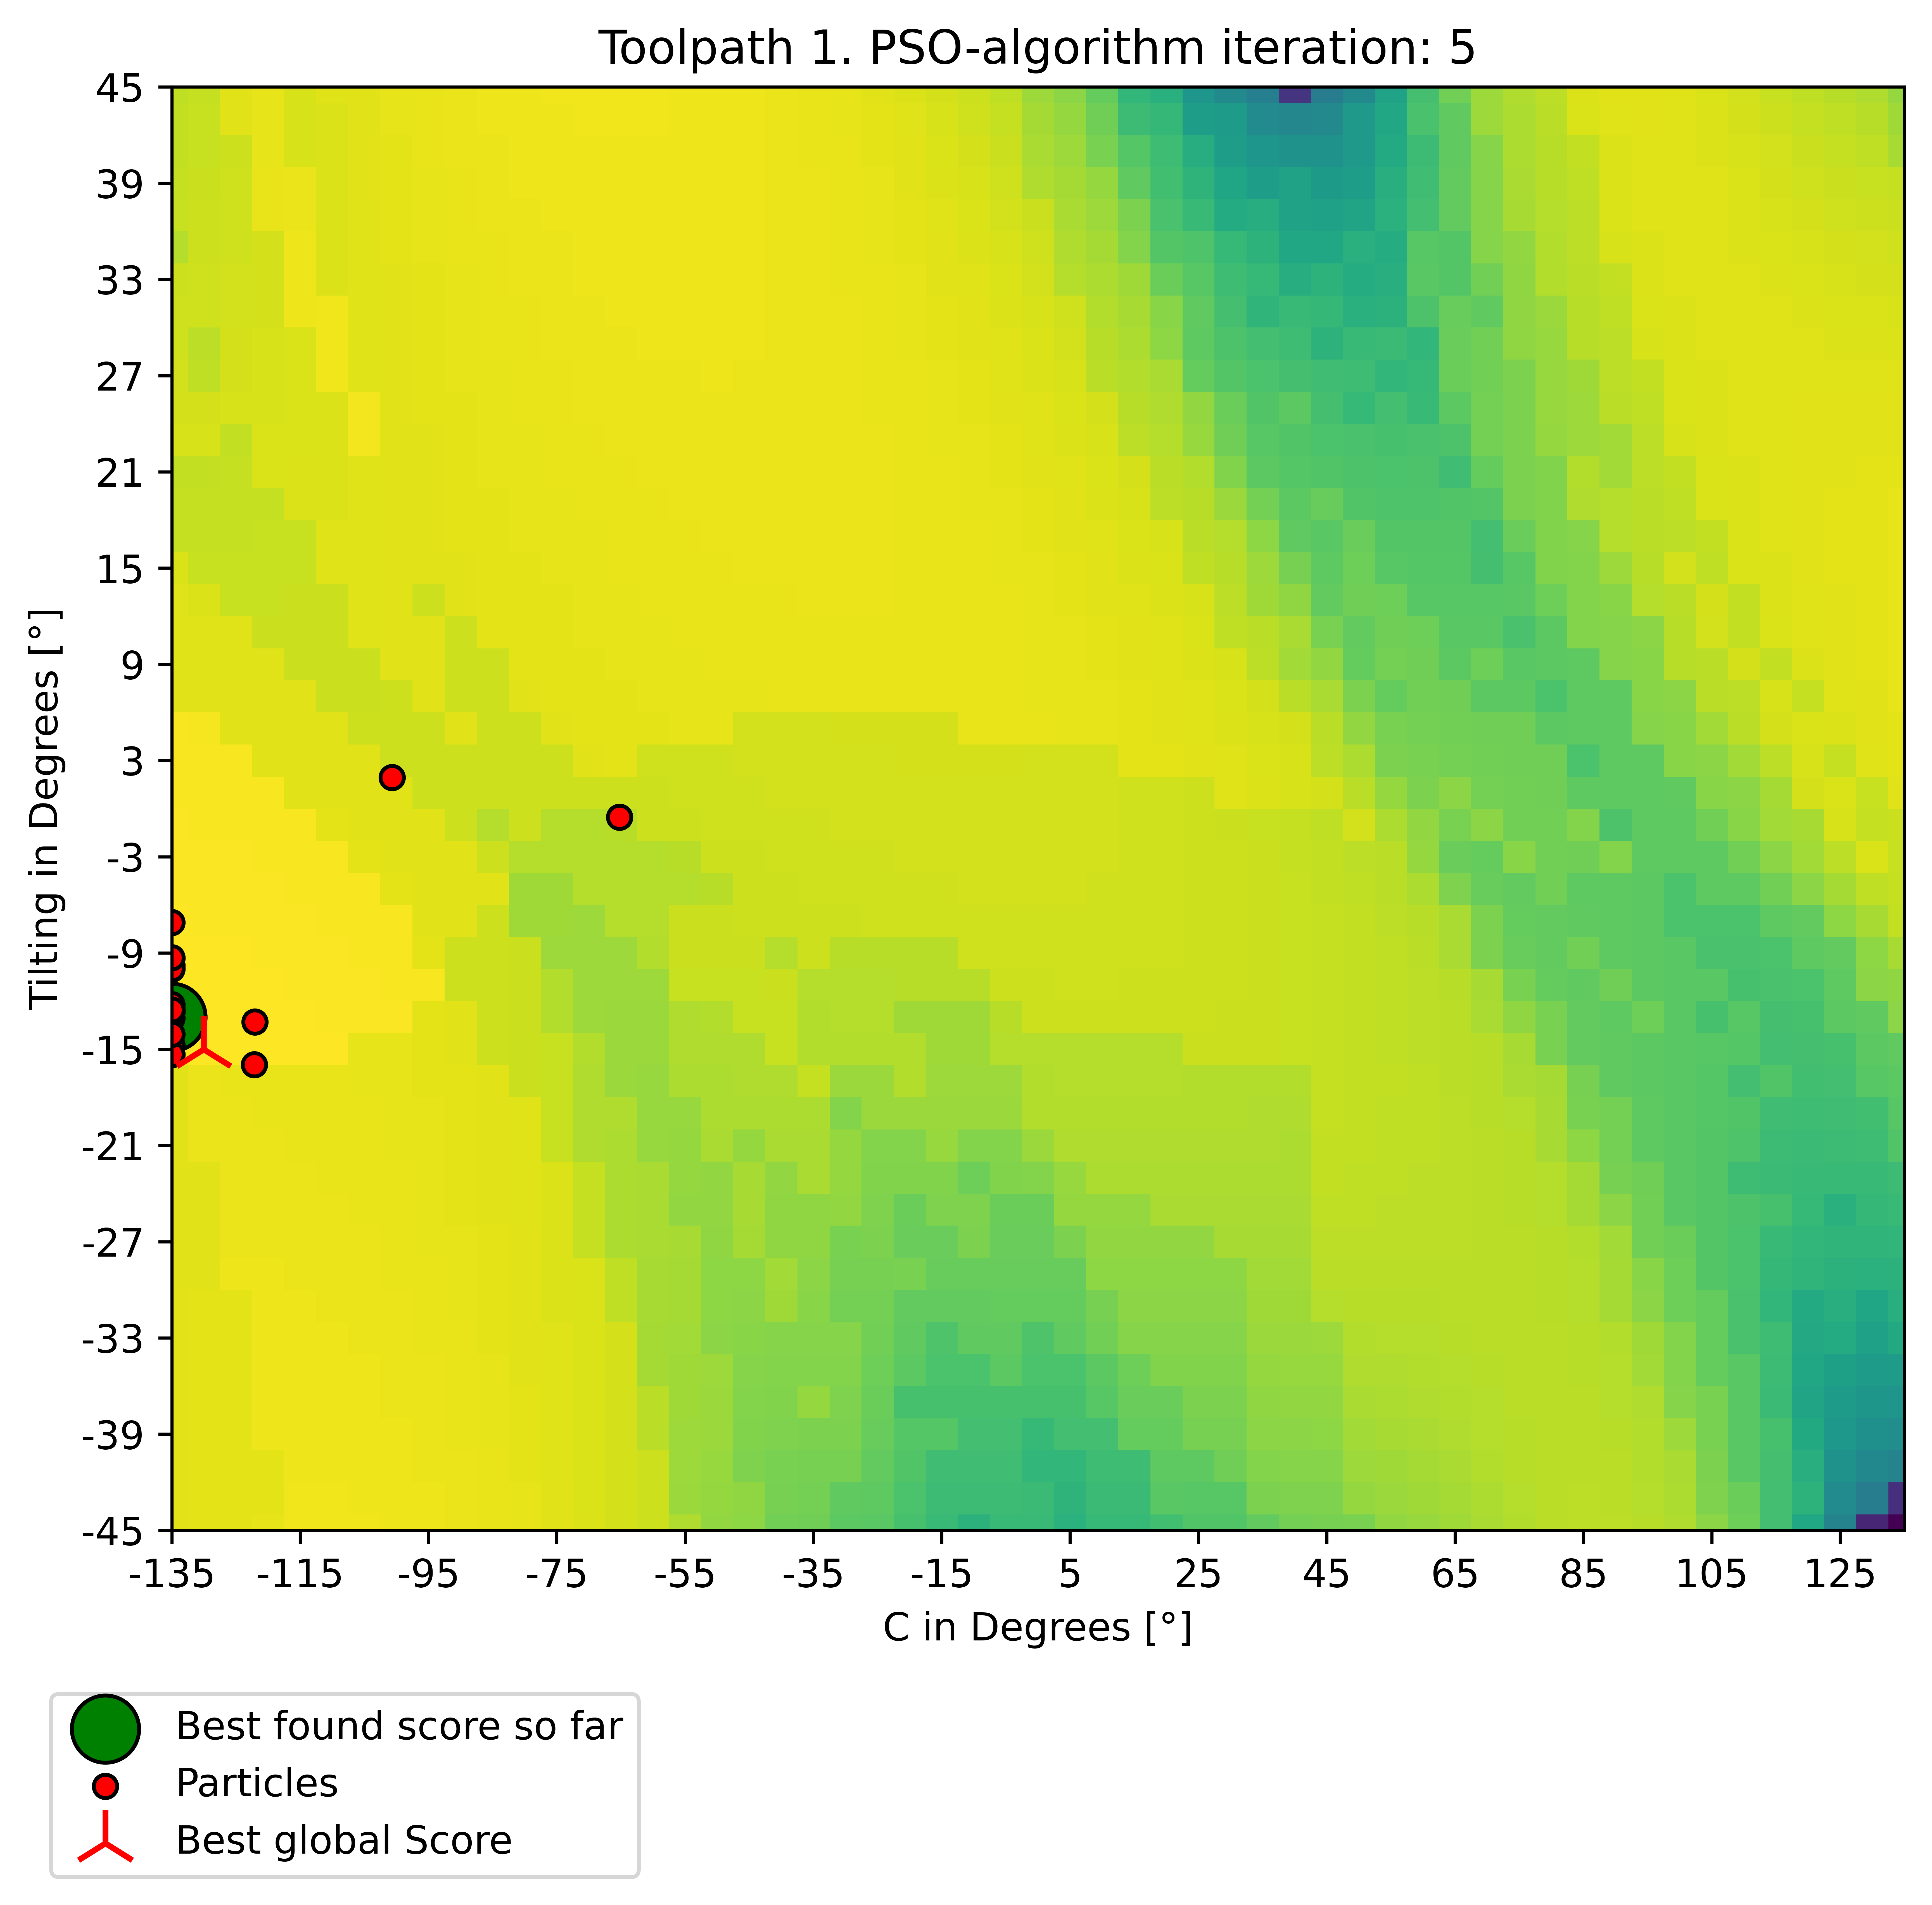
\includegraphics[width=\textwidth]{figures/swarm_true/1_5.png}
		\caption{PSO Iteration 5 on toolpath 1}
		\label{5_true_1}
	\end{minipage}\hfill
	\begin{minipage}{0.5\textwidth}
		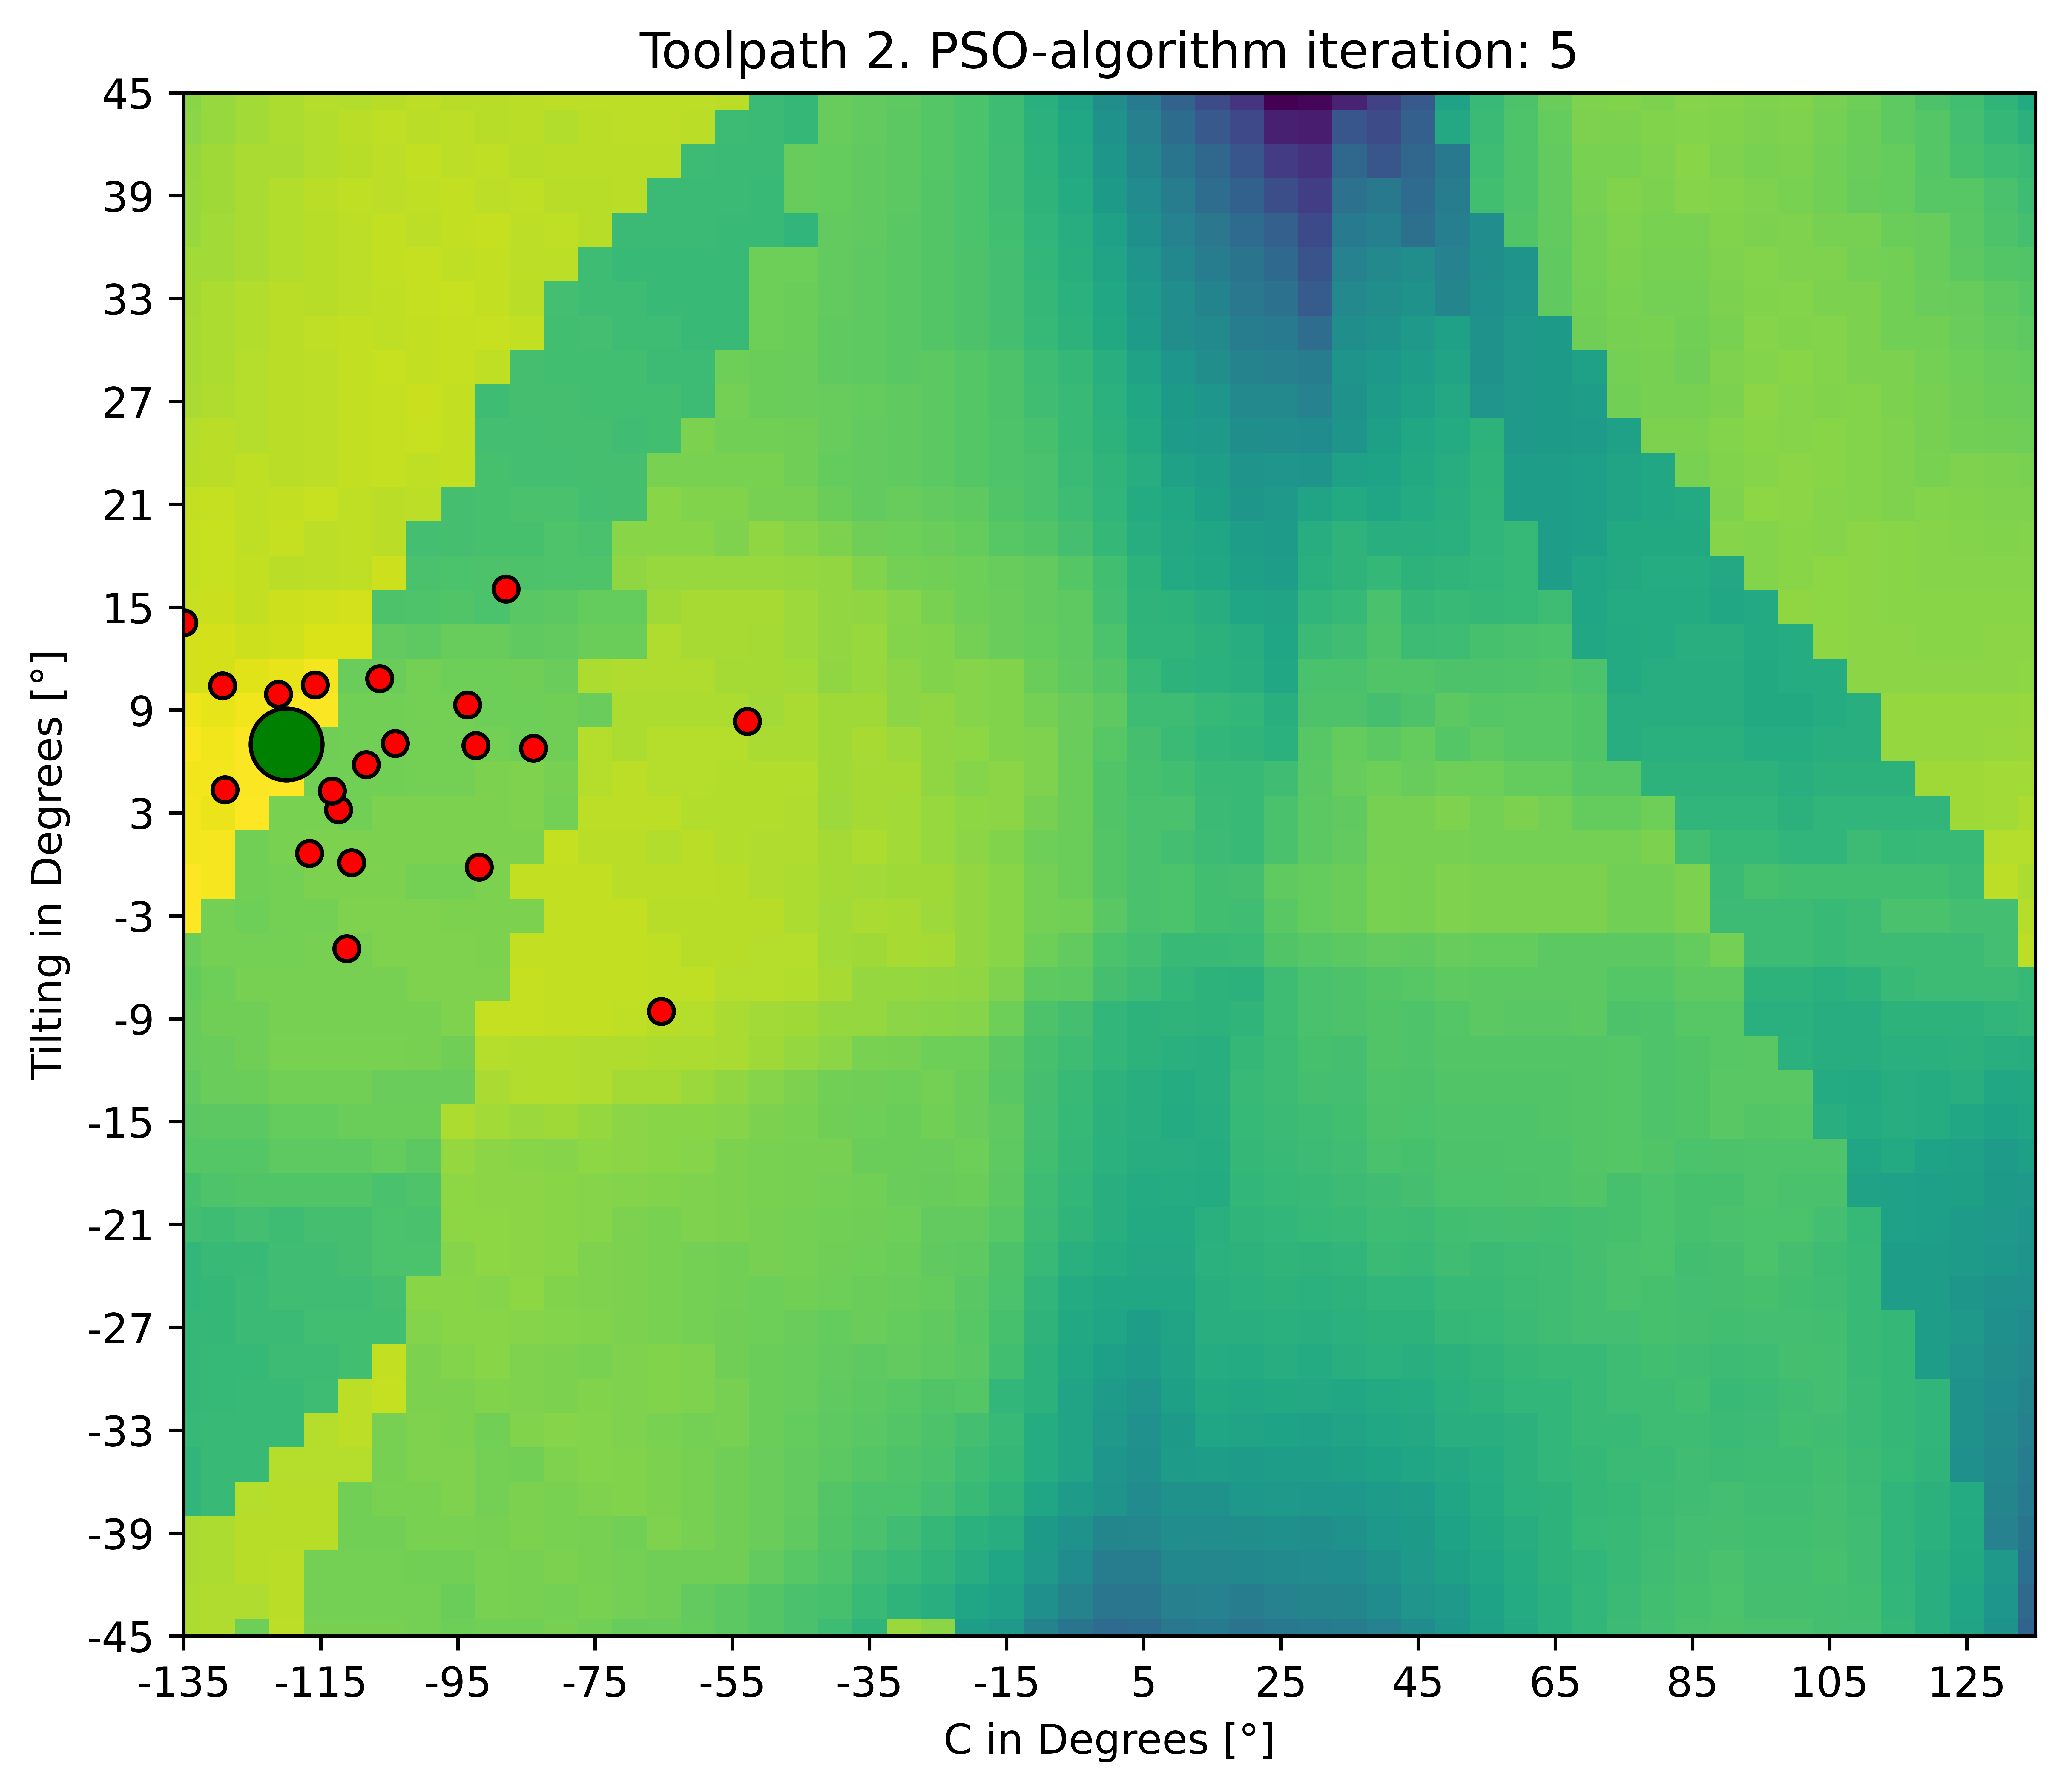
\includegraphics[width=\textwidth]{figures/swarm_true/2_5.png}
		\caption{PSO Iteration 5 on toolpath 2}
		\label{5_true_2}
	\end{minipage}\par
\end{figure}

\newpage
\section{Analysis and Discussion of the results}%
In the following the results are analyzed in more detail and critically discussed.

\subsection{Analysis}
\subsection{Discussion}%